\documentclass[10pt]{article}
\usepackage[margin=1in]{geometry}
 \usepackage{auto-pst-pdf}
\usepackage{graphicx}
%\usepackage{arydshln}
\usepackage{ifpdf}
\ifpdf
  \usepackage{epstopdf}
\fi
\usepackage{multirow}
\usepackage{epsfig}
\usepackage{float}
\usepackage{url}
\usepackage{color}
\usepackage{subfigure}

%\newcommand\solidrule[1][1cm]{\rule[0.5ex]{#1}{.4pt}}
%\newcommand\dashedrule{\mbox{%
%  \solidrule[2mm]\hspace{2mm}\solidrule[2mm]\hspace{2mm}\solidrule[2mm]}}
  
%\usepackage{hyperref}

\begin{document}
\title{Empirical Check of Machine Homogeneity on Timing Protocol}

\author{
Young-Kyoon Suh\\
}
\maketitle

\section{Description}
In this work we do a check to see if the result on the same experiment is different 
on different nodes, each with the same machine specification.

\section{Experiment Notes}
We provide a short description of our experimental runs. 
In these experiments we used four nodes ({\tt sodb8}, {\tt sodb9}, {\tt sodb10}, and {\tt sodb12} ) 
in the same cluster. 

%% done
\begin{table}[h]
\begin{center}
\begin{tabular}{|p{2cm}|p{3cm}|p{6cm}|p{4cm}|} \hline
Machine & Task Length & Description & Time Length\\ \hline
{\tt sodb8} &  INC1$\sim$INC128 & Runs of 300 samples & 2017-02-09 $\sim$ 2017-02-10\\ \hline
{\tt sodb9} &  INC1$\sim$INC128 & Runs of 300 samples & 2017-02-09 $\sim$ 2017-02-10\\ \hline
{\tt sodb10} & INC1$\sim$INC128 & Runs of 300 samples & 2017-02-09 $\sim$ 2017-02-10\\ \hline
{\tt sodb12} & INC1$\sim$INC128 & Runs of 300 samples & 2017-02-09 $\sim$ 2017-02-10\\ \hline
\end{tabular}
\end{center}
\vspace{-.2in}
\caption{Detailed description of INC data used for histograms\label{tab:exp_notes}}
\end{table}

\paragraph{Measurement Quality Across the SoDB Nodes:} 
Fig.~\ref{fig:machine_comp} shows 
the standard deviation and relative error of 
elapsed time (ET) and process time (PT) on the different SoDB nodes 
as the task length of INC increases. 

\begin{figure}[t]
	\centering
	\subfigure[Standard Deviation - ET]{
		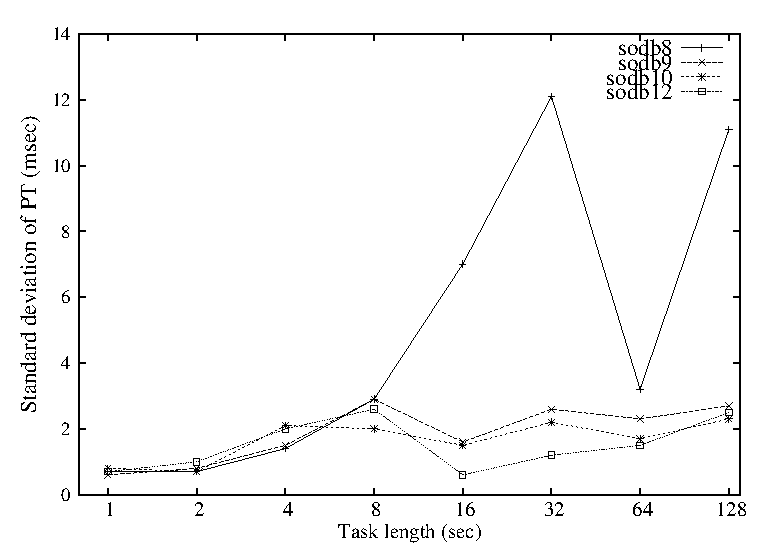
\includegraphics[scale=0.6]{overall/machine_et_std.eps}
        \label{fig:pt_std}
    }
    \subfigure[Relative Error - ET]{
        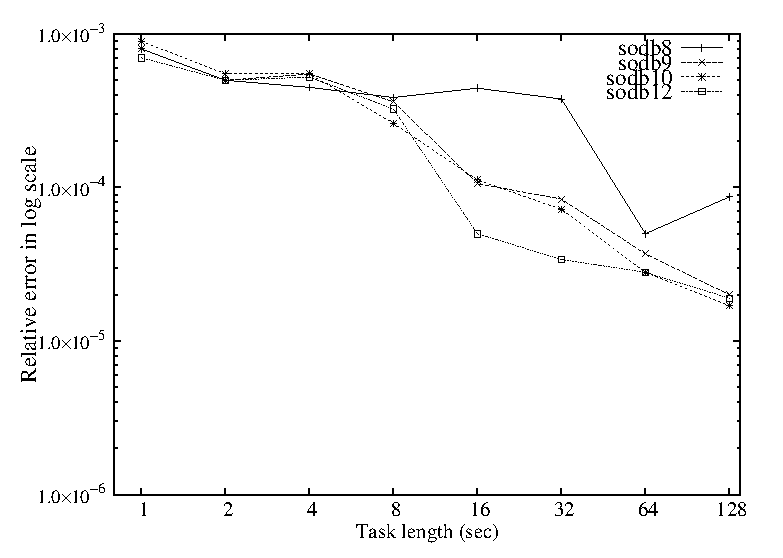
\includegraphics[scale=0.6]{overall/machine_et_re.eps}
        \label{fig:pt_re}
    }
	\subfigure[Standard Deviation - PT]{
		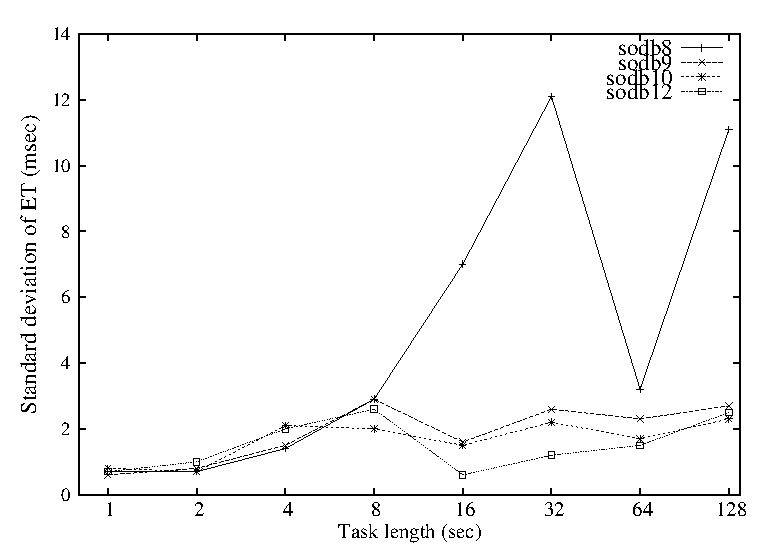
\includegraphics[scale=0.6]{overall/machine_pt_std.eps}
        \label{fig:pt_std}
    }
    \subfigure[Relative Error - PT]{
        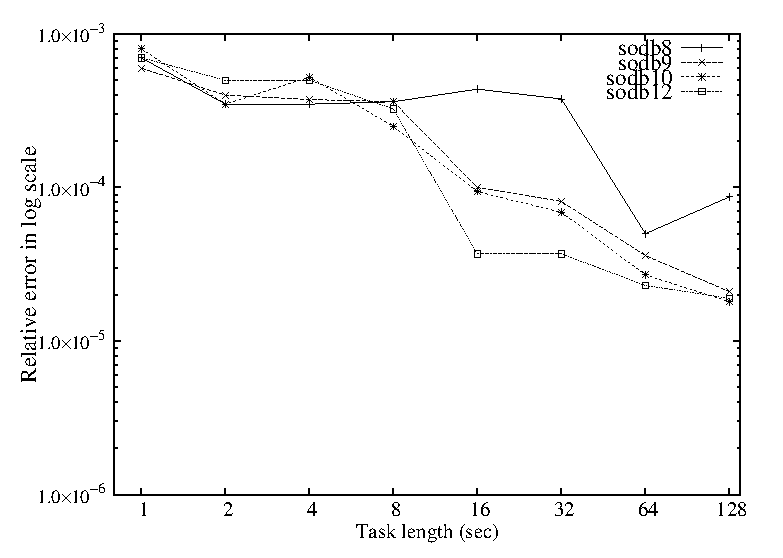
\includegraphics[scale=0.6]{overall/machine_pt_re.eps}
        \label{fig:pt_re}
    }
    \caption{Measurement Quality Comparison among Different SoDB Machines}
    \label{fig:machine_comp}
\end{figure}

\newpage

Each of the following sections exhibits histograms of ET and PT 
over increasing INC's task lengths on each individual node. 

\newpage

\subsection{{\tt sodb12}~\label{sec:sodb12_hist}} 
This section exhibits histograms on the EMPv5 data obtained on {\tt sodb12}. 
The detailed description of the base data are from Table~\ref{tab:exp_notes}.

\subsubsection{ET}

\begin{figure}[hp!]
	\centering
	\subfigure[ET frequency on INC1 on {\tt sodb12}]{
		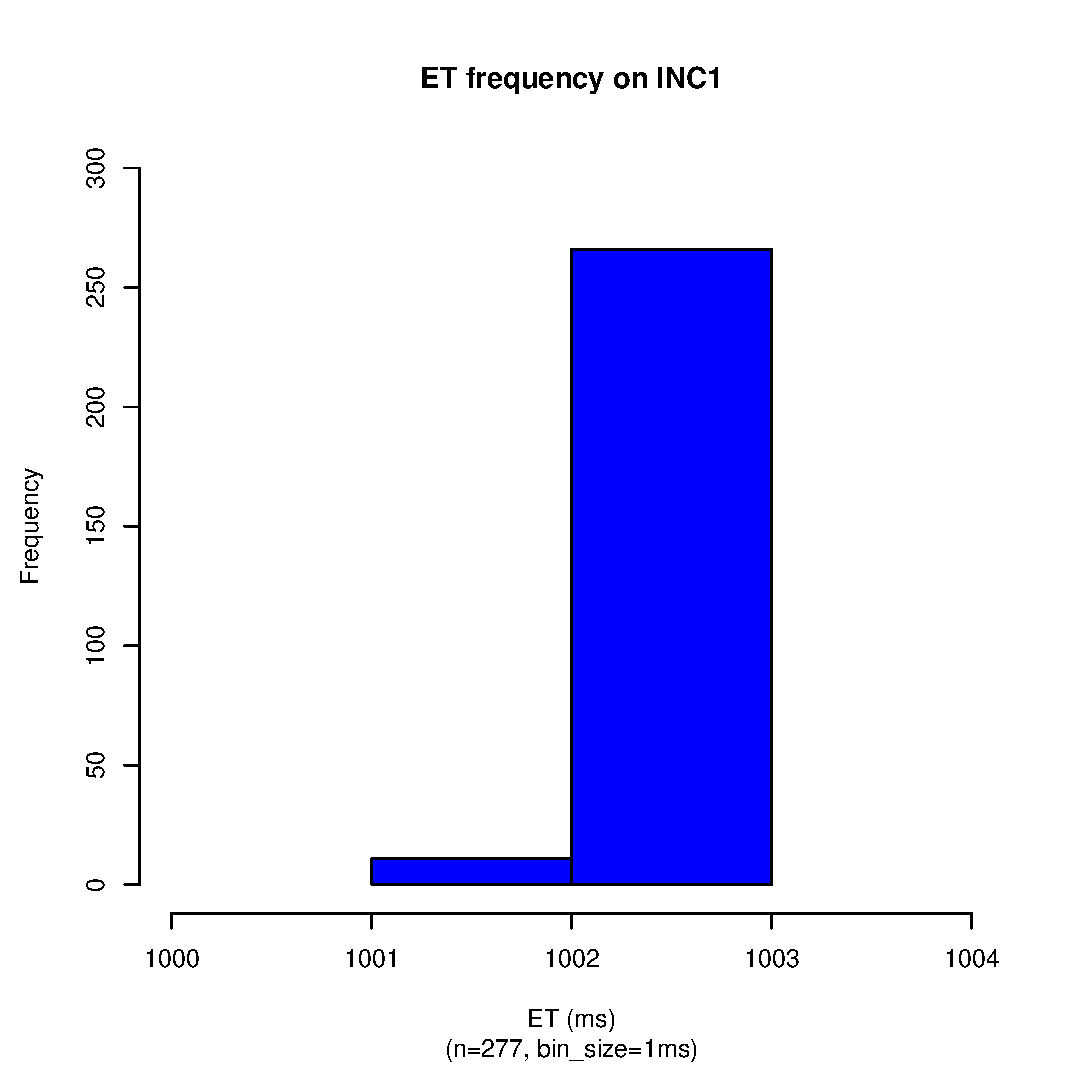
\includegraphics[scale=0.43]{sodb12/1_sec_et_hist_v5.eps}
		\label{fig:s12_inc1_et_hist_v5}
	}
	\subfigure[ET frequency on INC2 on {\tt sodb12}]{
		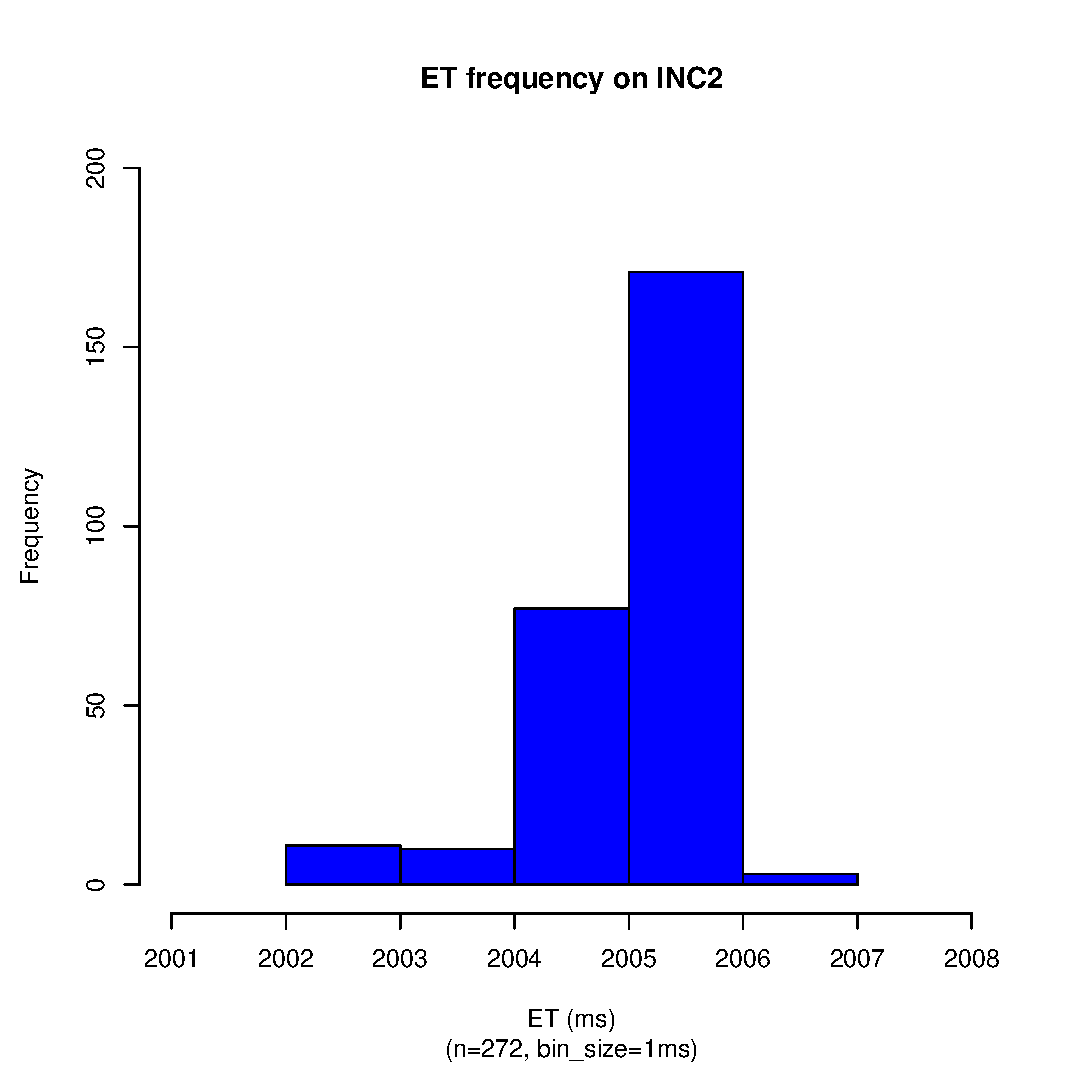
\includegraphics[scale=0.43]{sodb12/2_sec_et_hist_v5.eps}
		\label{fig:s12_inc2_et_hist_v5}
	}
	\subfigure[ET frequency on INC4 on {\tt sodb12}]{
		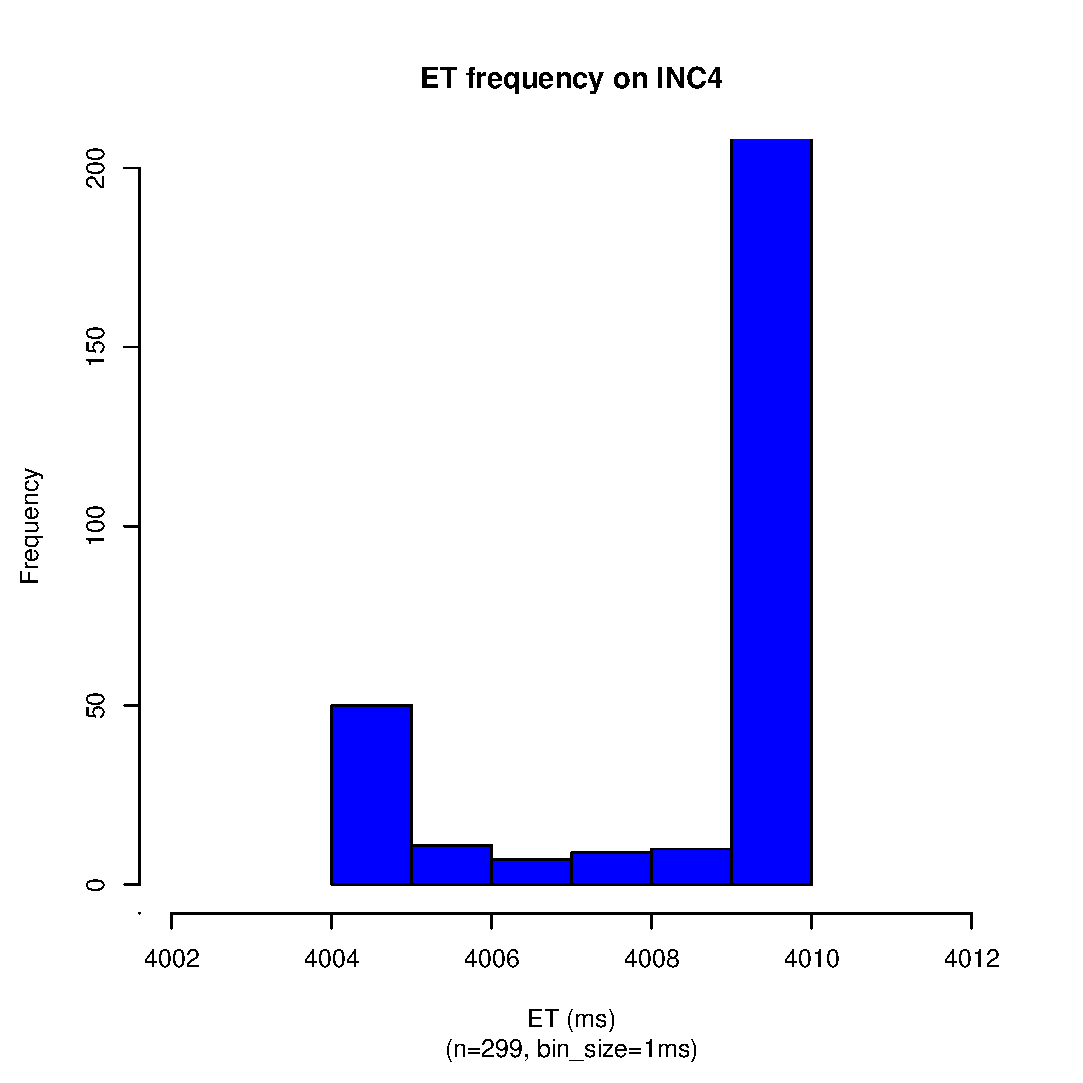
\includegraphics[scale=0.43]{sodb12/4_sec_et_hist_v5.eps}
		\label{fig:s12_inc4_et_hist_v5}
	}
	\subfigure[ET frequency on INC8 on {\tt sodb12}]{
		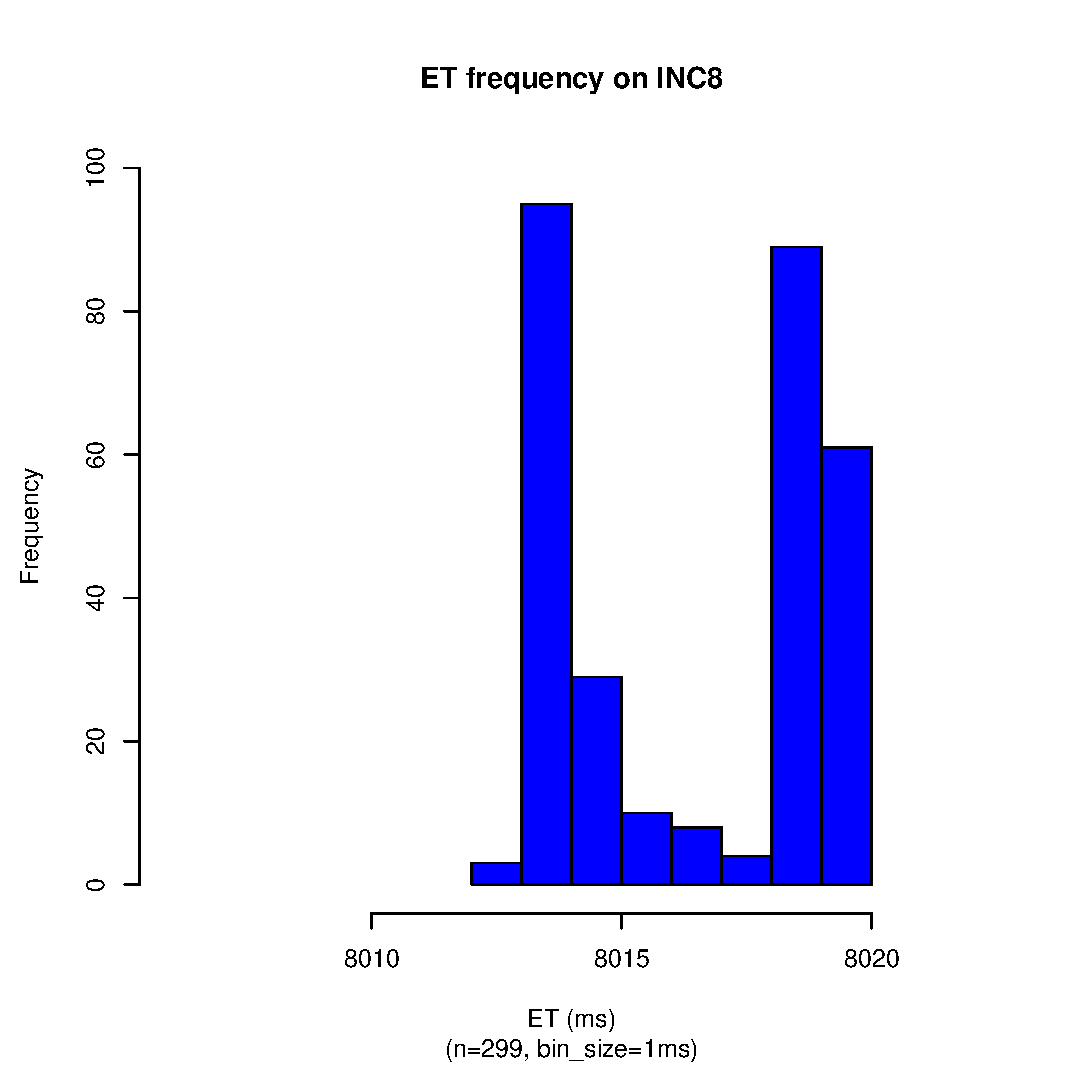
\includegraphics[scale=0.43]{sodb12/8_sec_et_hist_v5.eps}
		\label{fig:s12_inc8_et_hist_v5}
	}
	\caption{ET Histograms of INC1 ... INC8~\label{fig:s12_et_hist1}}
\end{figure}

\begin{figure}[hp!]
	\centering
	\subfigure[ET frequency on INC16 on {\tt sodb12}]{
		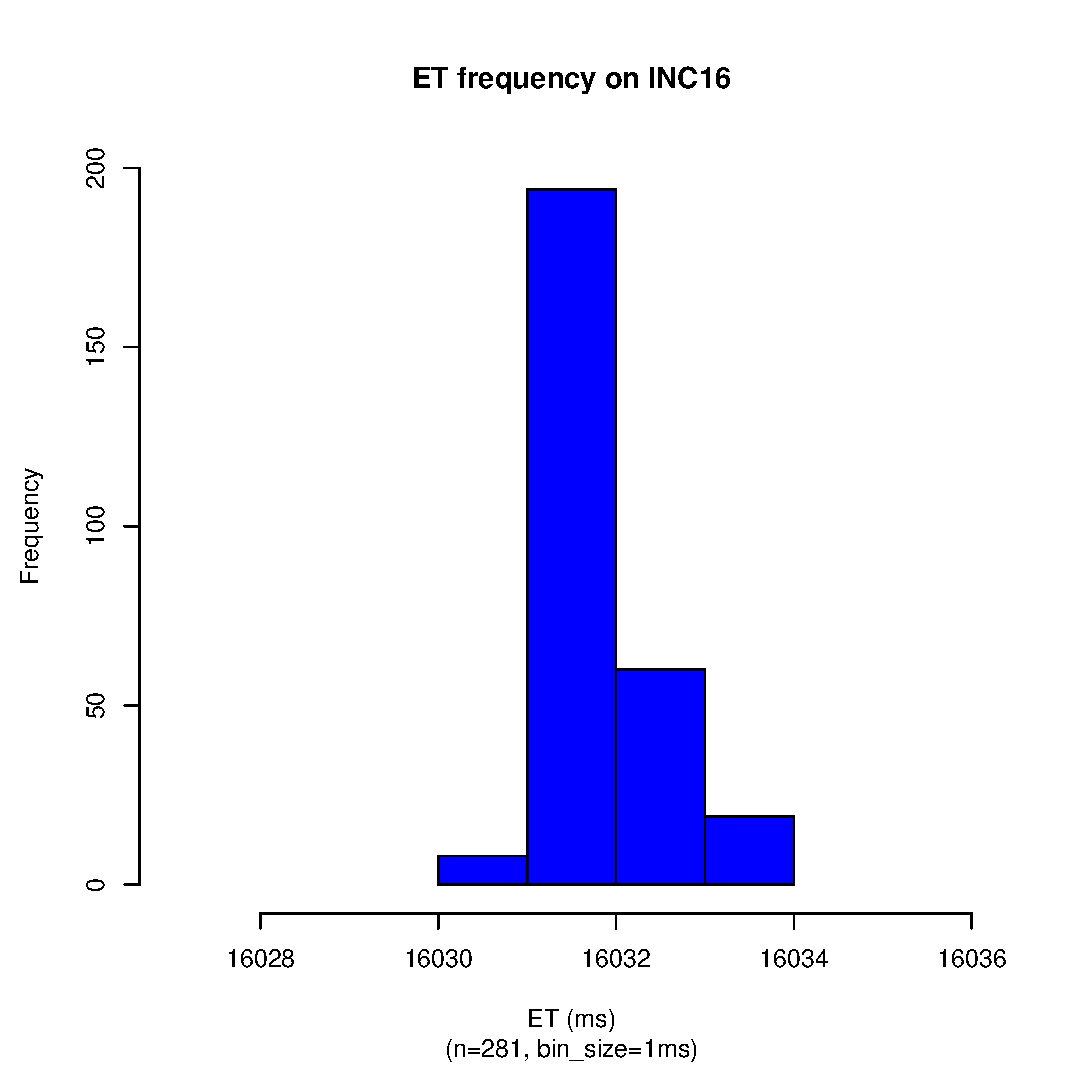
\includegraphics[scale=0.43]{sodb12/16_sec_et_hist_v5.eps}
		\label{fig:s12_inc16_et_hist_v5}
	}
	\subfigure[ET frequency on INC32 on {\tt sodb12}]{
		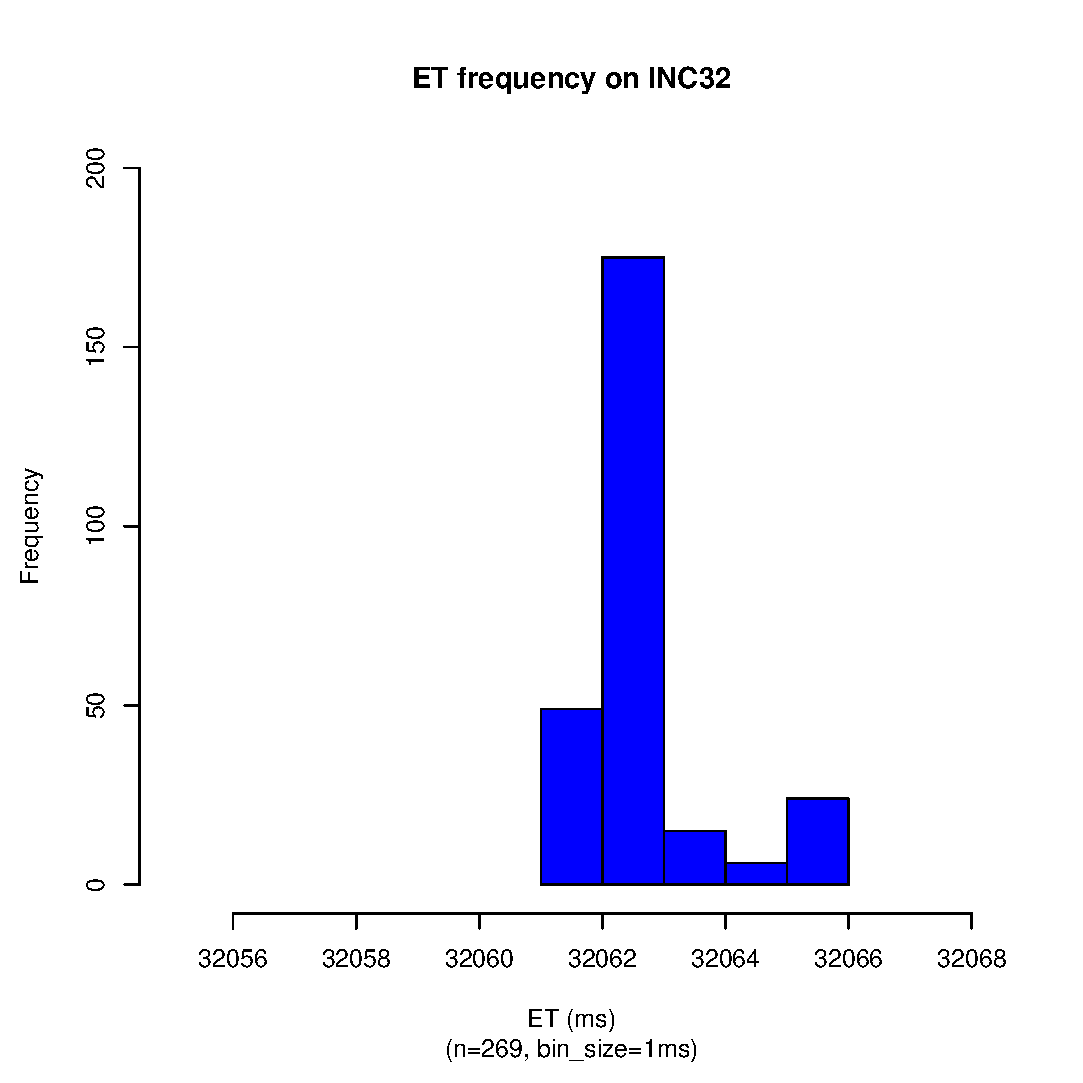
\includegraphics[scale=0.43]{sodb12/32_sec_et_hist_v5.eps}
		\label{fig:s12_inc32_et_hist_v5}
	}
	\subfigure[ET frequency on INC64 on {\tt sodb12}]{
		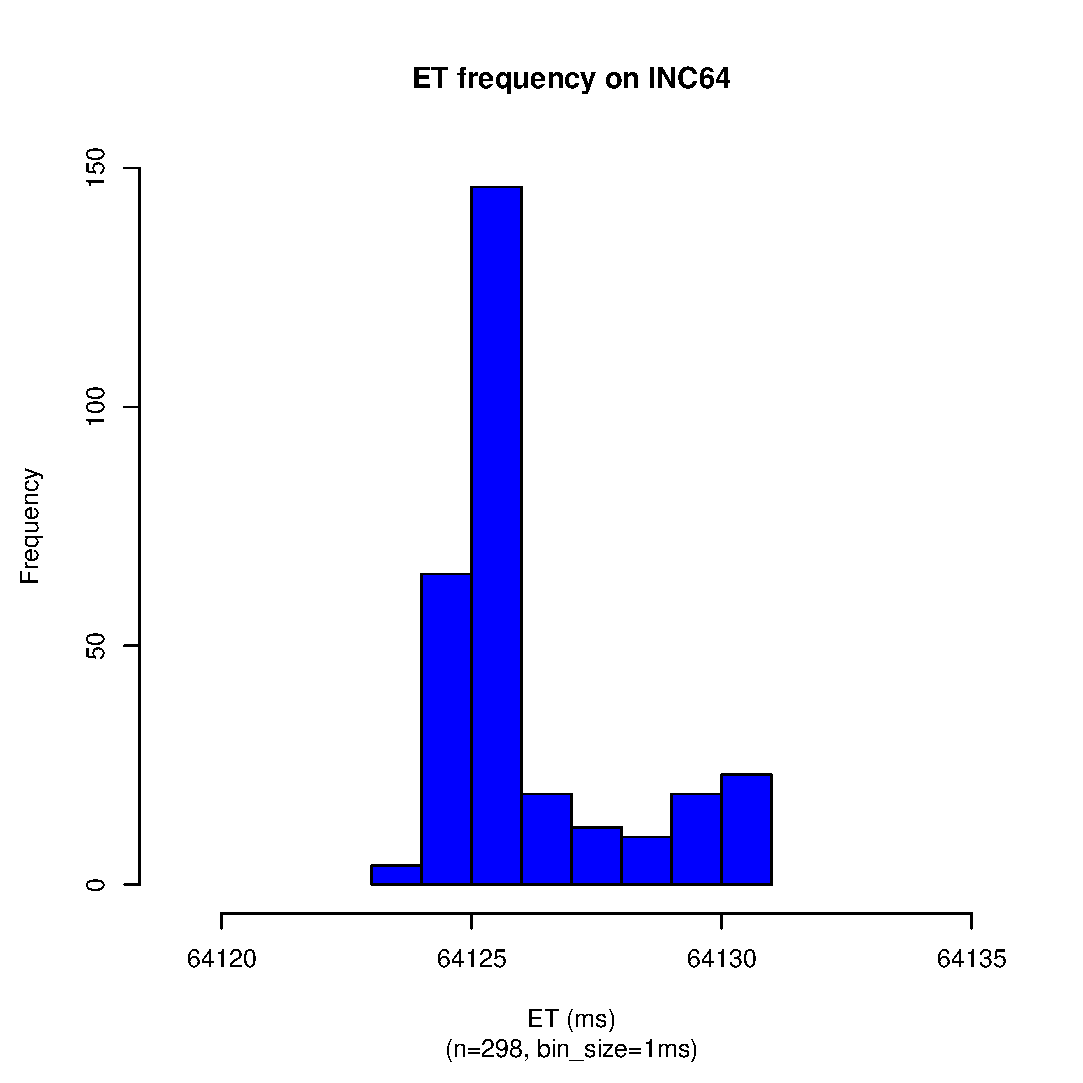
\includegraphics[scale=0.43]{sodb12/64_sec_et_hist_v5.eps}
		\label{fig:s12_inc64_et_hist_v5}
	}
	\subfigure[ET frequency on INC128 on {\tt sodb12}]{
		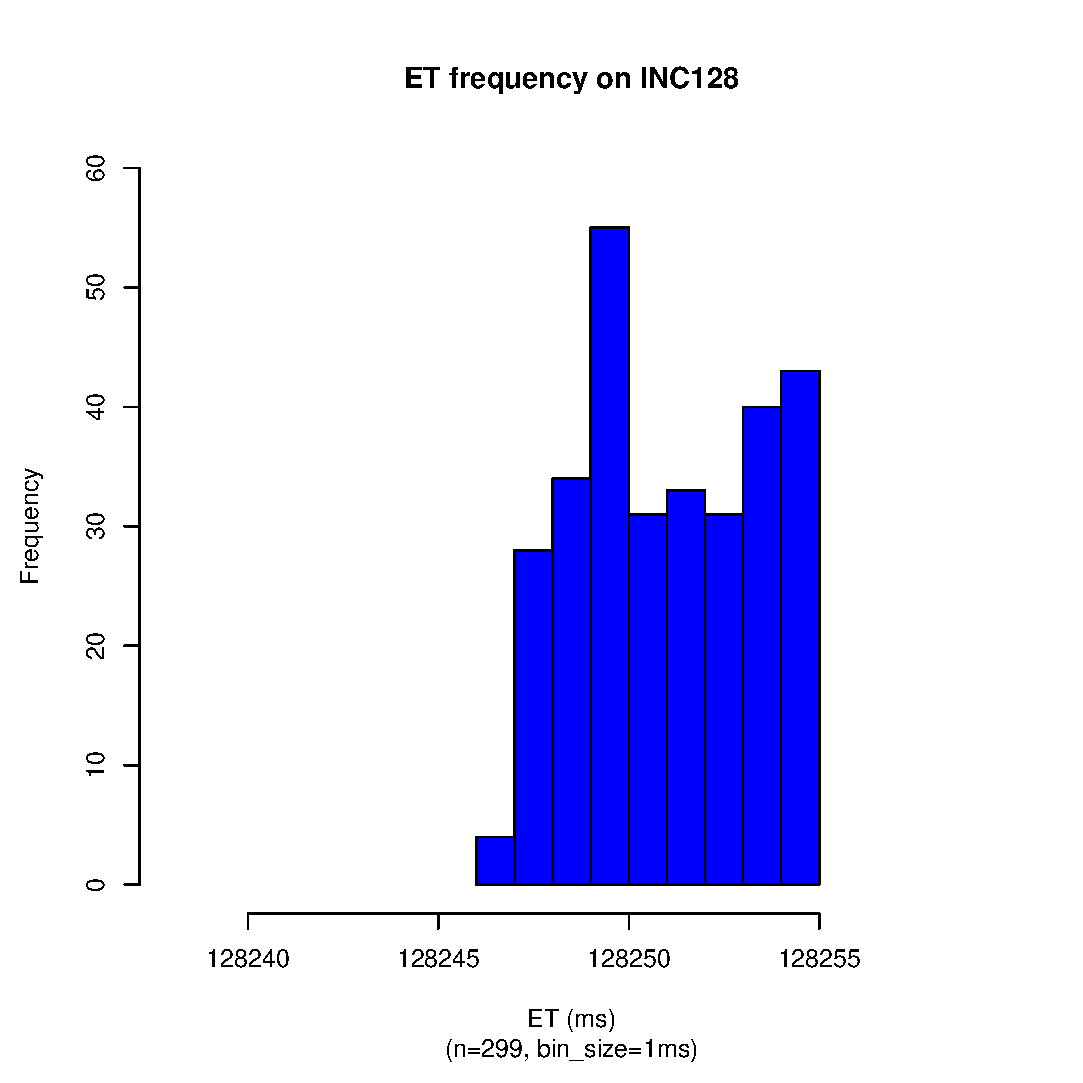
\includegraphics[scale=0.43]{sodb12/128_sec_et_hist_v5.eps}
		\label{fig:s12_inc128_et_hist_v5}
	}
	\caption{ET Histograms of INC16 ... INC128~\label{fig:s12_et_hist2}}
\end{figure}

\newpage

\subsubsection{PT}

\begin{figure}[hp!]
	\centering
	\subfigure[PT frequency on INC1 on {\tt sodb12}]{
		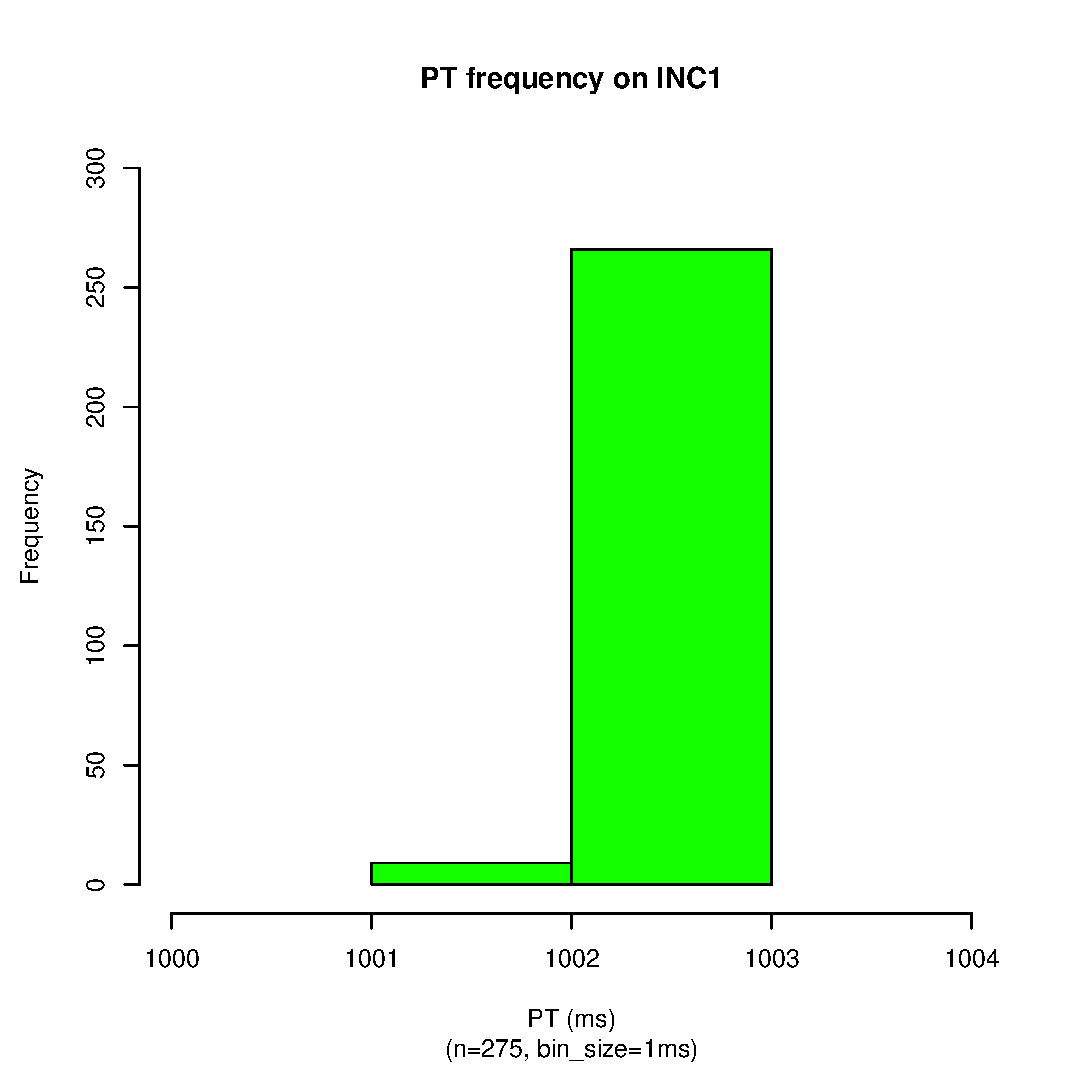
\includegraphics[scale=0.43]{sodb12/1_sec_pt_hist_v5.eps}
		\label{fig:s12_inc1_hist_v5}
	}
	\subfigure[PT frequency on INC2 on {\tt sodb12}]{
		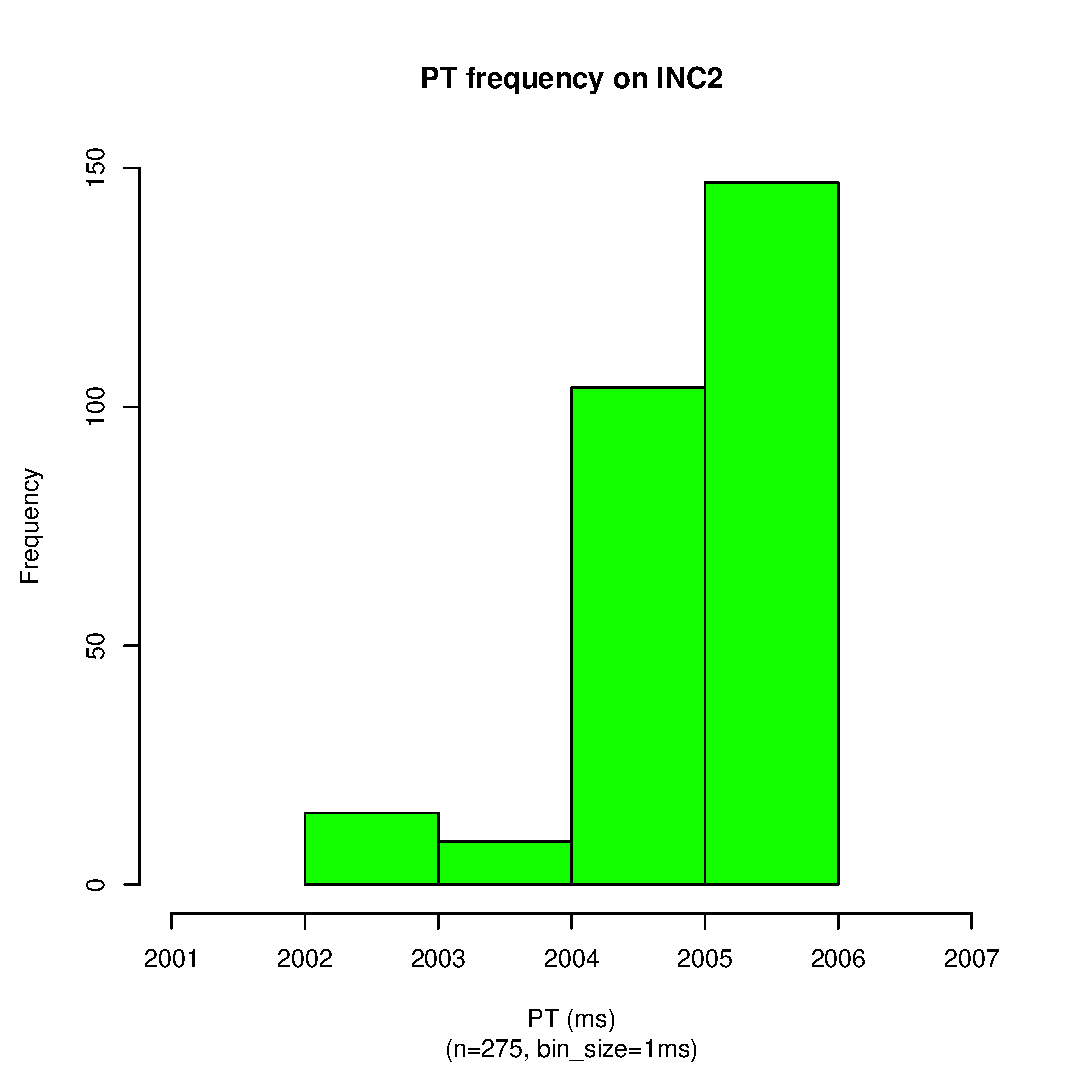
\includegraphics[scale=0.43]{sodb12/2_sec_pt_hist_v5.eps}
		\label{fig:s12_inc2_hist_v5}
	}
	\subfigure[PT frequency on INC4 on {\tt sodb12}]{
		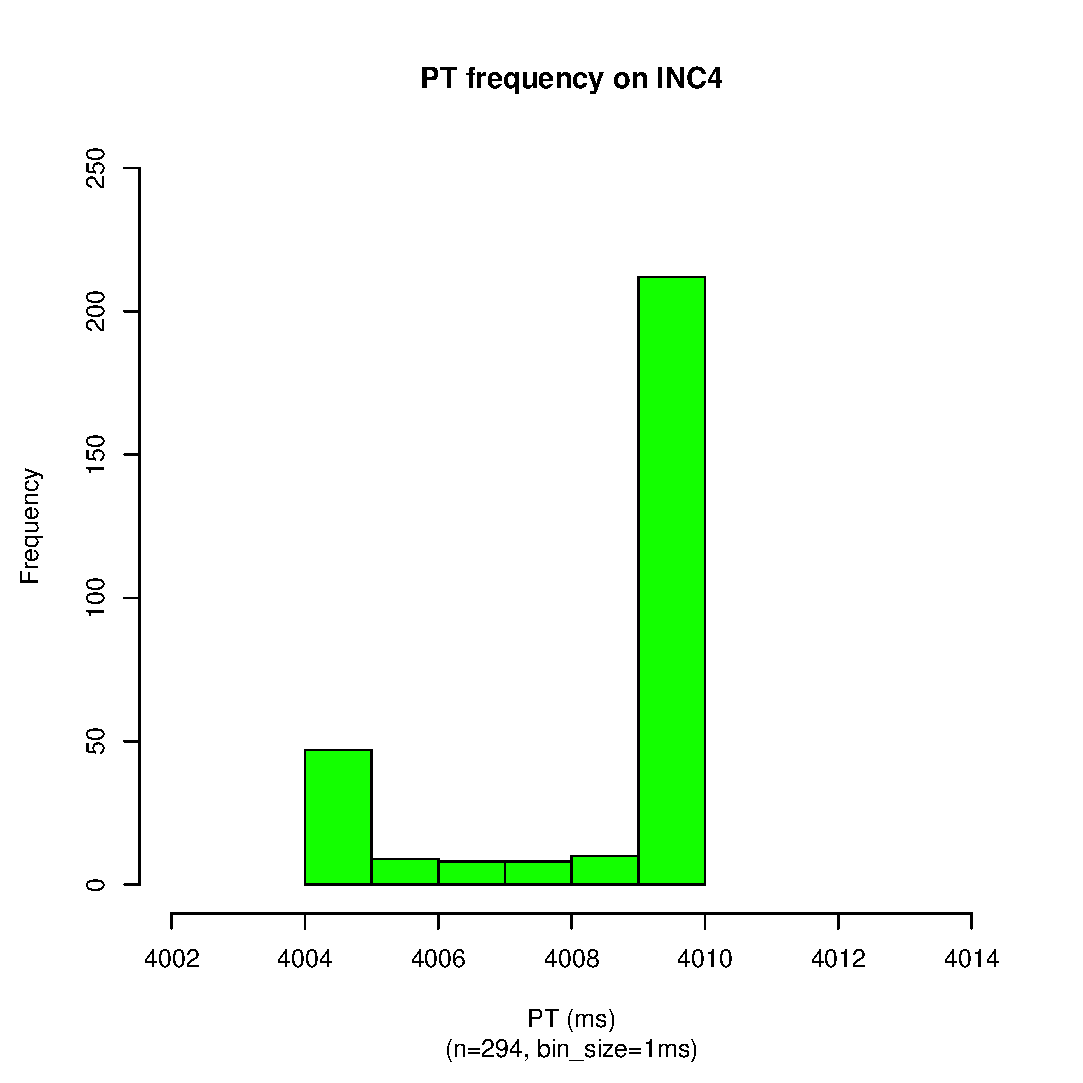
\includegraphics[scale=0.43]{sodb12/4_sec_pt_hist_v5.eps}
		\label{fig:s12_inc4_hist_v5}
	}
	\subfigure[PT frequency on INC8 on {\tt sodb12}]{
		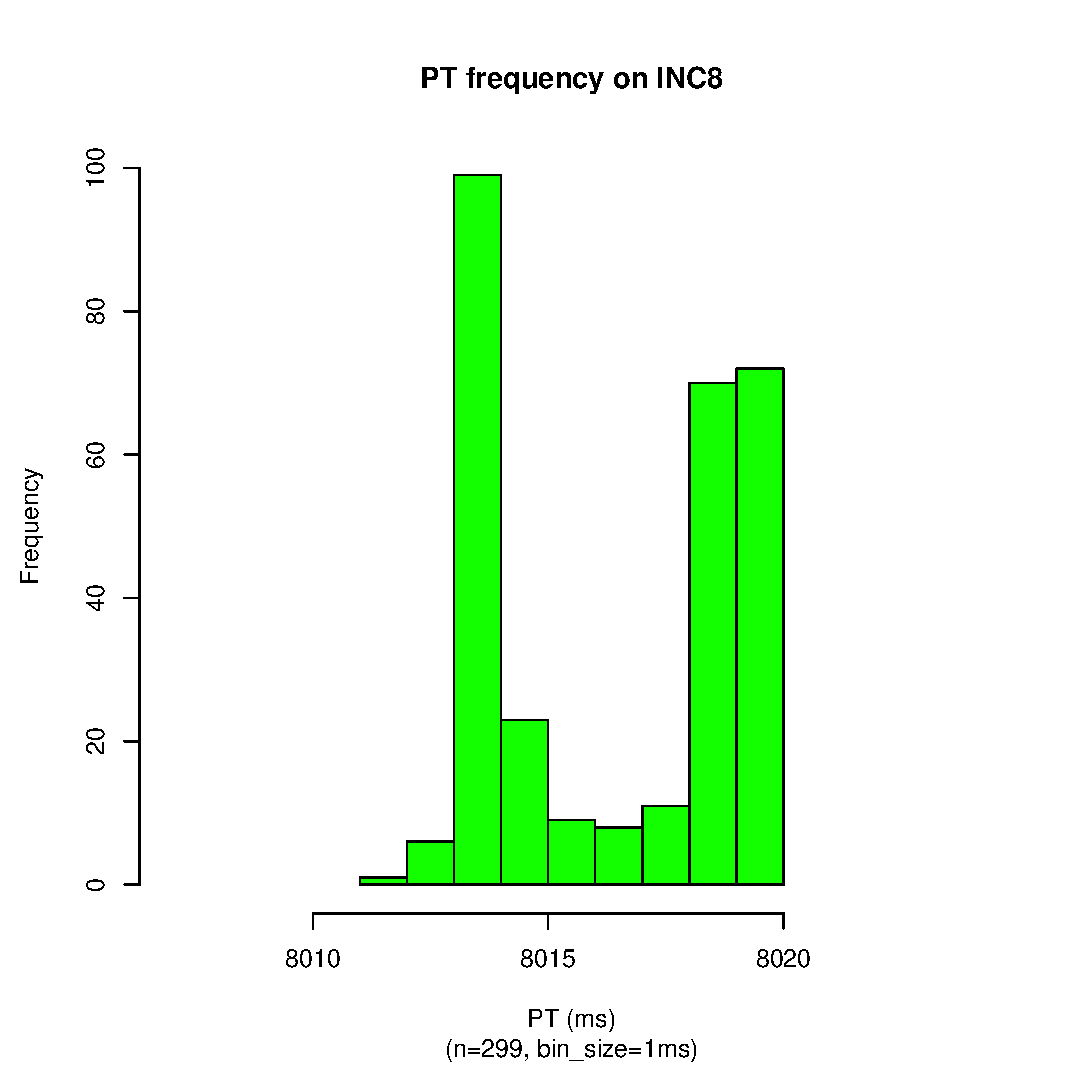
\includegraphics[scale=0.43]{sodb12/8_sec_pt_hist_v5.eps}
		\label{fig:s12_inc8_hist_v5}
	}
	\caption{PT Histograms of INC1 ... INC8~\label{fig:s12_pt_hist1}}
\end{figure}

\begin{figure}[hp!]
	\centering
	\subfigure[PT frequency on INC16 on {\tt sodb12}]{
		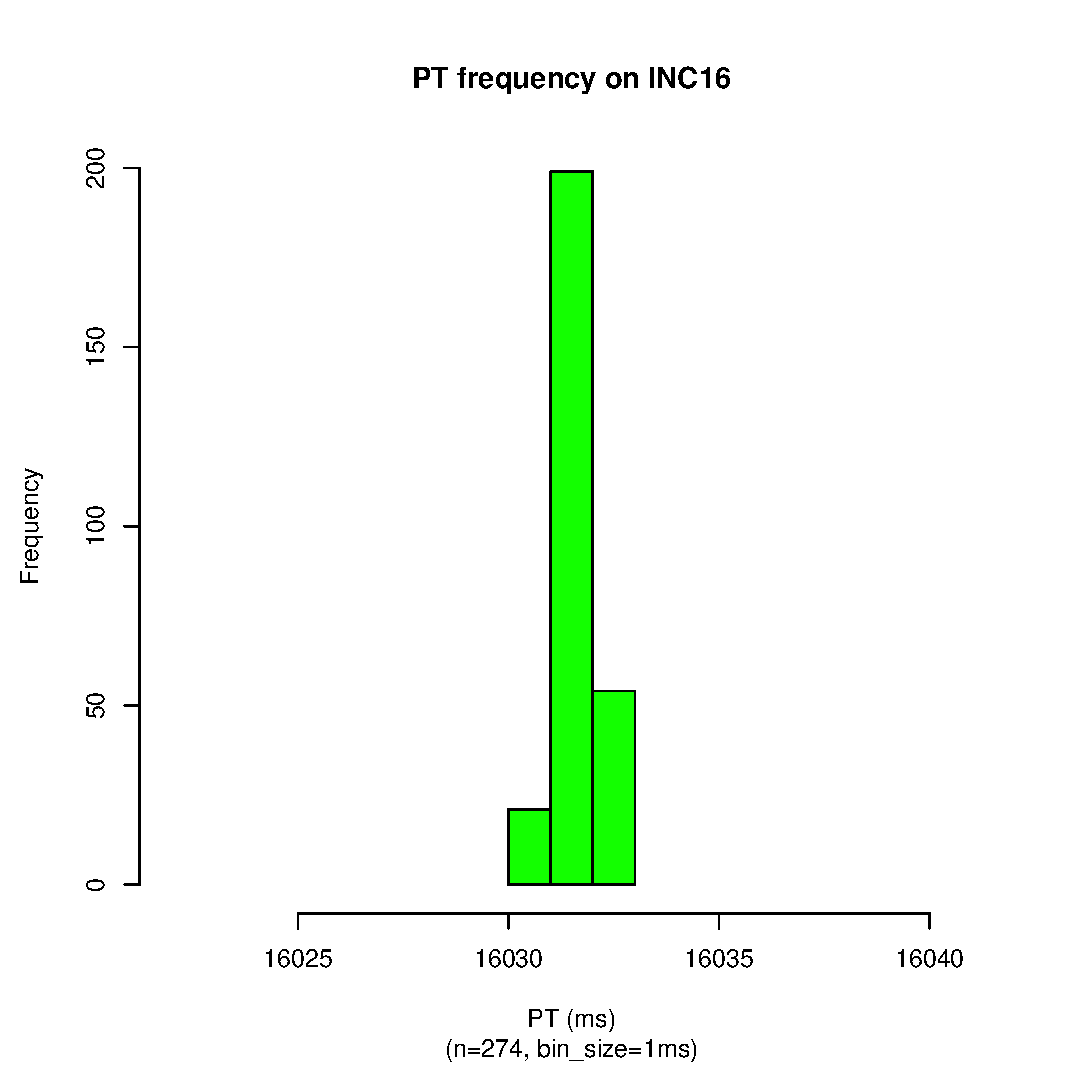
\includegraphics[scale=0.43]{sodb12/16_sec_pt_hist_v5.eps}
		\label{fig:s12_inc16_hist_v5}
	}
	\subfigure[PT frequency on INC32 on {\tt sodb12}]{
		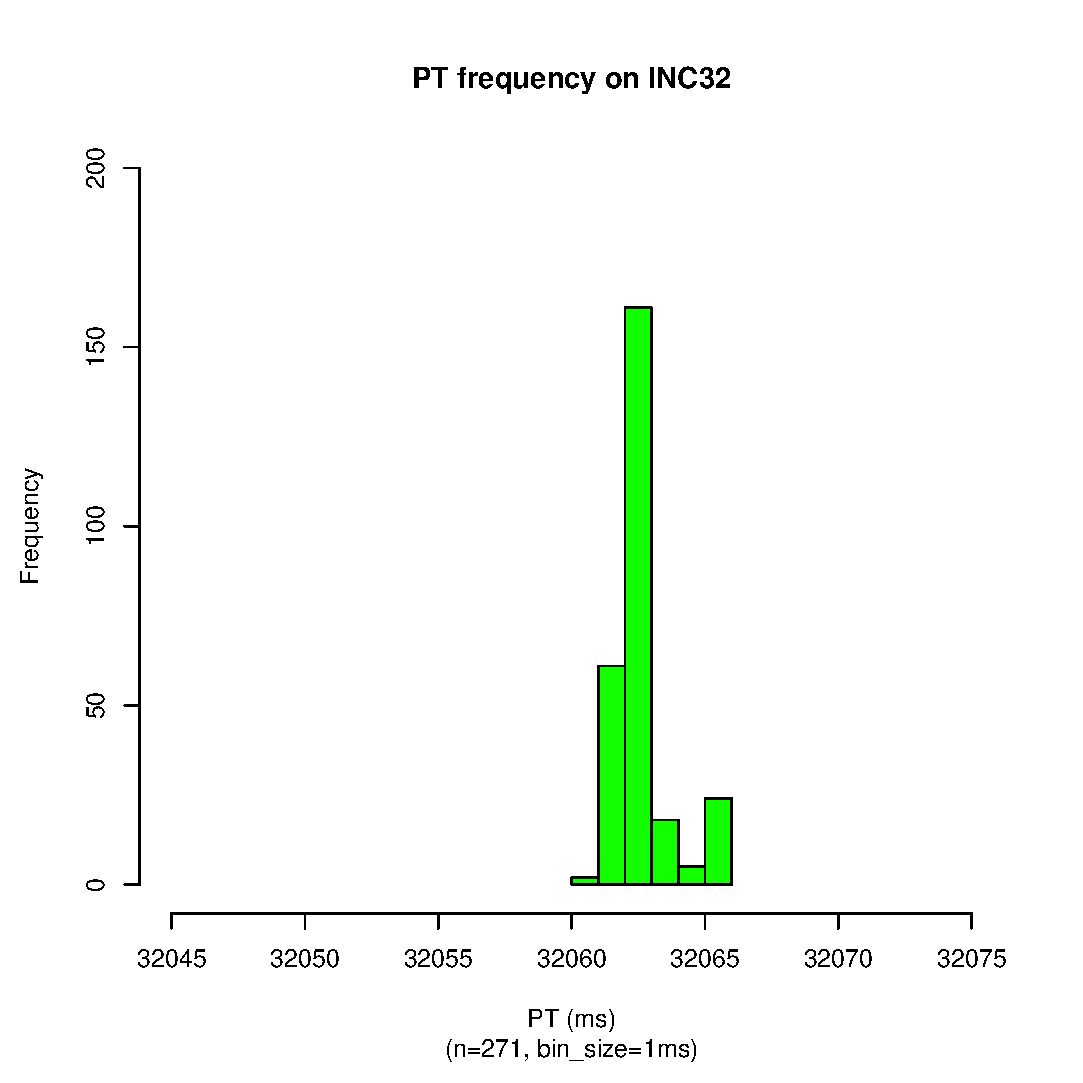
\includegraphics[scale=0.43]{sodb12/32_sec_pt_hist_v5.eps}
		\label{fig:s12_inc32_hist_v5}
	}
	\subfigure[PT frequency on INC64 on {\tt sodb12}]{
		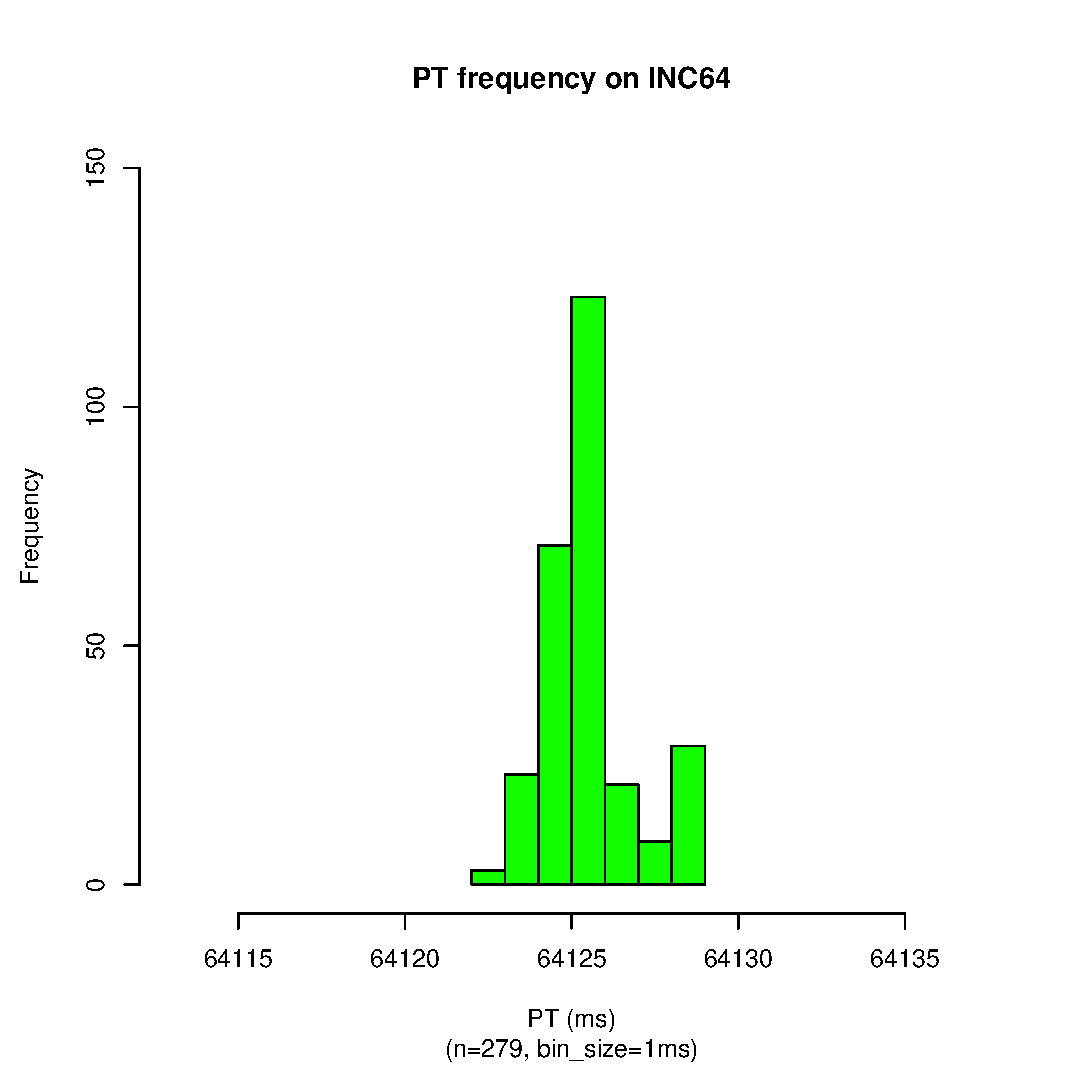
\includegraphics[scale=0.43]{sodb12/64_sec_pt_hist_v5.eps}
		\label{fig:s12_inc64_hist_v5}
	}
	\subfigure[PT frequency on INC128 on {\tt sodb12}]{
		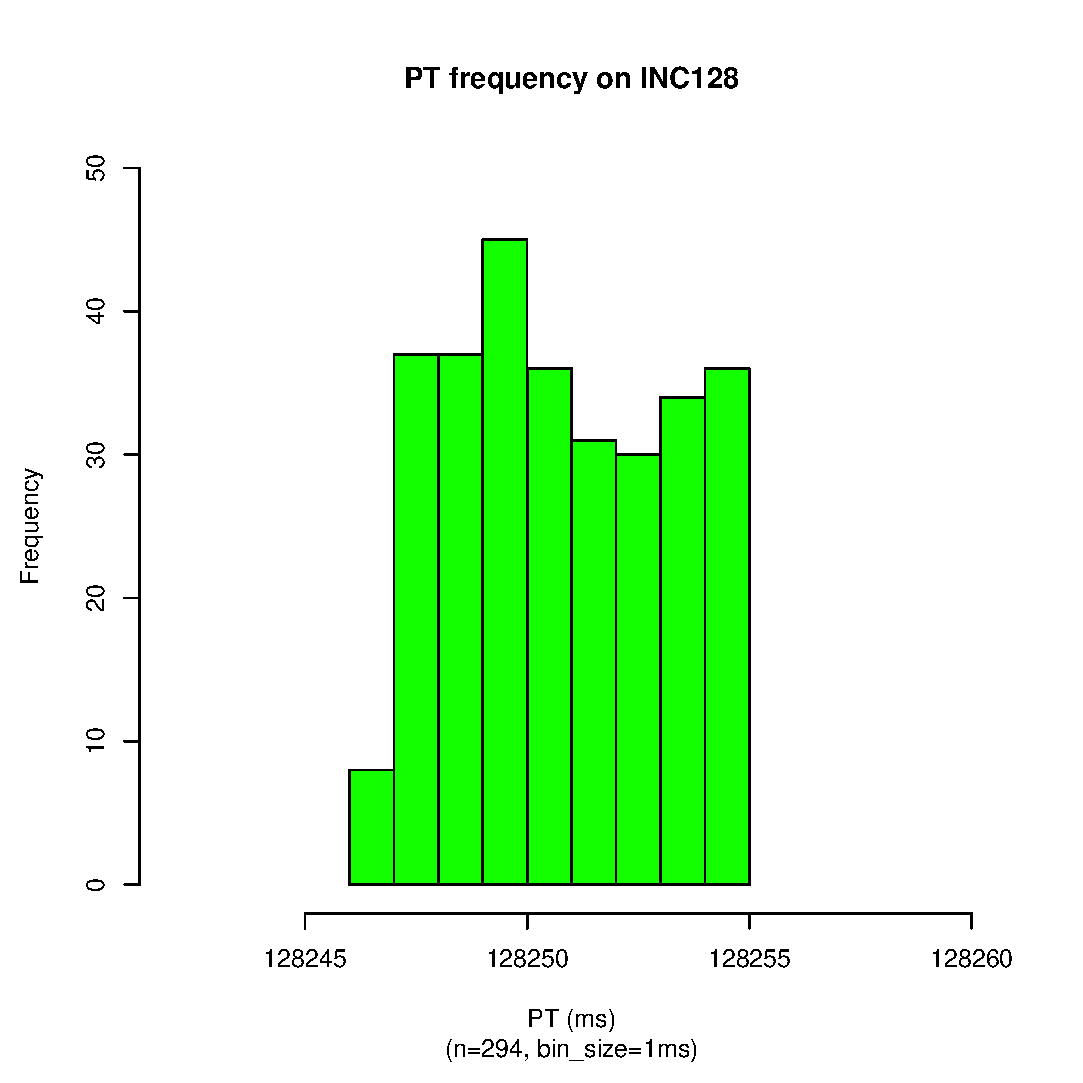
\includegraphics[scale=0.43]{sodb12/128_sec_pt_hist_v5.eps}
		\label{fig:s12_inc128_hist_v5}
	}
	\caption{PT Histograms of INC16 ... INC64~\label{fig:s12_pt_hist2}}
\end{figure}
\newpage

\subsection{{\tt sodb12}~\label{sec:sodb12_hist}} 
This section exhibits histograms on the EMPv5 data obtained on {\tt sodb12}. 
The detailed description of the base data are from Table~\ref{tab:exp_notes}.

\subsubsection{ET}

\begin{figure}[hp!]
	\centering
	\subfigure[ET frequency on INC1 on {\tt sodb12}]{
		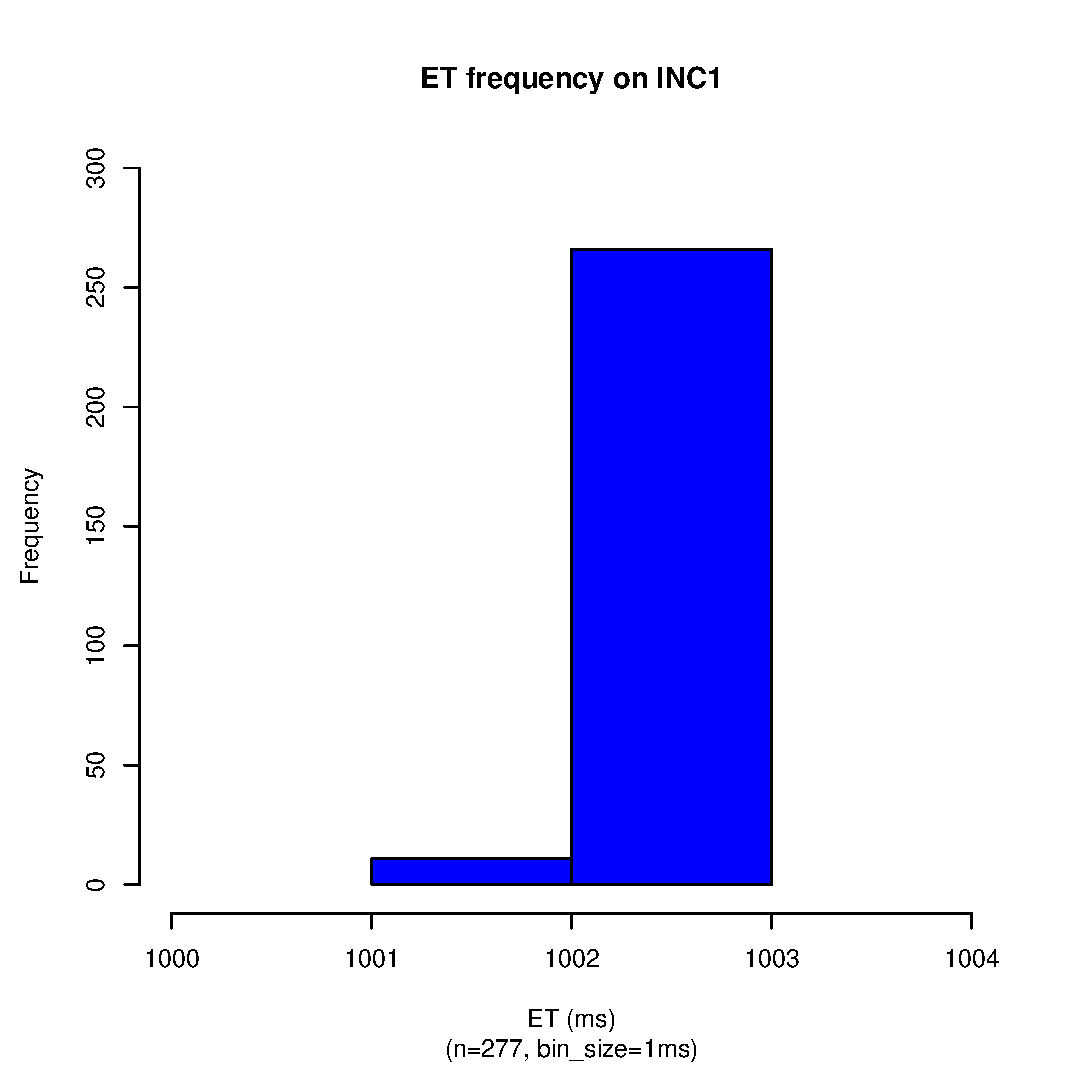
\includegraphics[scale=0.43]{sodb12/1_sec_et_hist_v5.eps}
		\label{fig:s12_inc1_et_hist_v5}
	}
	\subfigure[ET frequency on INC2 on {\tt sodb12}]{
		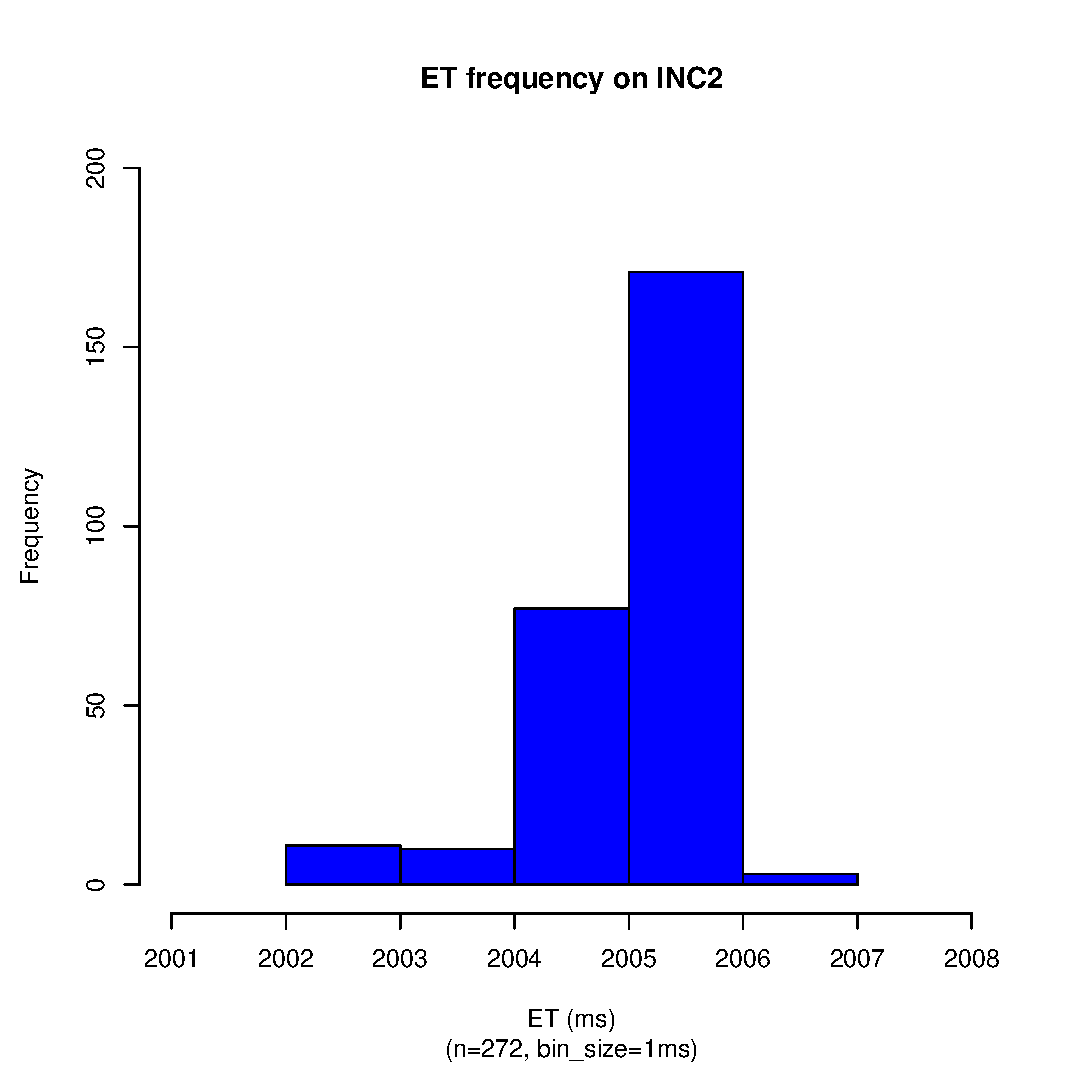
\includegraphics[scale=0.43]{sodb12/2_sec_et_hist_v5.eps}
		\label{fig:s12_inc2_et_hist_v5}
	}
	\subfigure[ET frequency on INC4 on {\tt sodb12}]{
		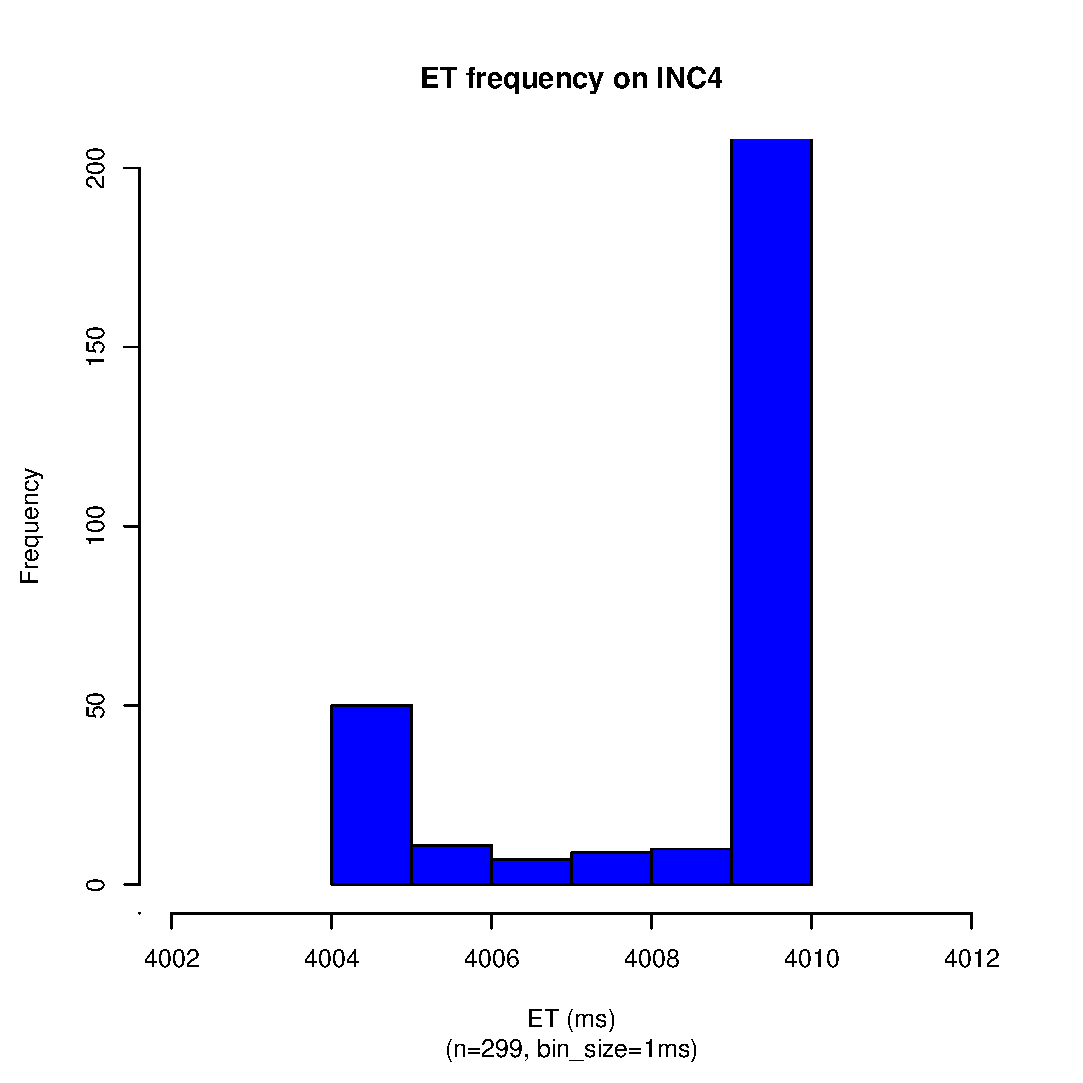
\includegraphics[scale=0.43]{sodb12/4_sec_et_hist_v5.eps}
		\label{fig:s12_inc4_et_hist_v5}
	}
	\subfigure[ET frequency on INC8 on {\tt sodb12}]{
		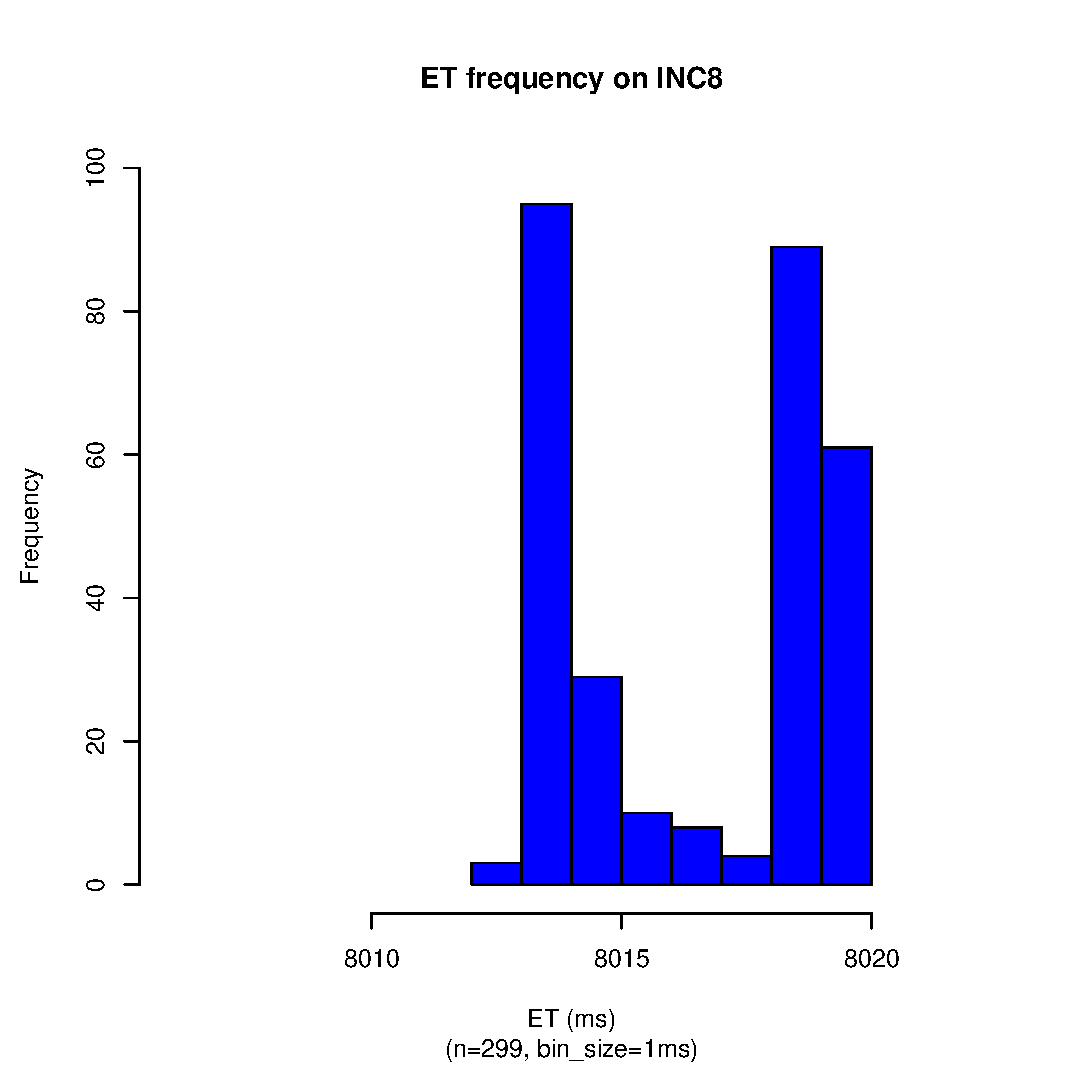
\includegraphics[scale=0.43]{sodb12/8_sec_et_hist_v5.eps}
		\label{fig:s12_inc8_et_hist_v5}
	}
	\caption{ET Histograms of INC1 ... INC8~\label{fig:s12_et_hist1}}
\end{figure}

\begin{figure}[hp!]
	\centering
	\subfigure[ET frequency on INC16 on {\tt sodb12}]{
		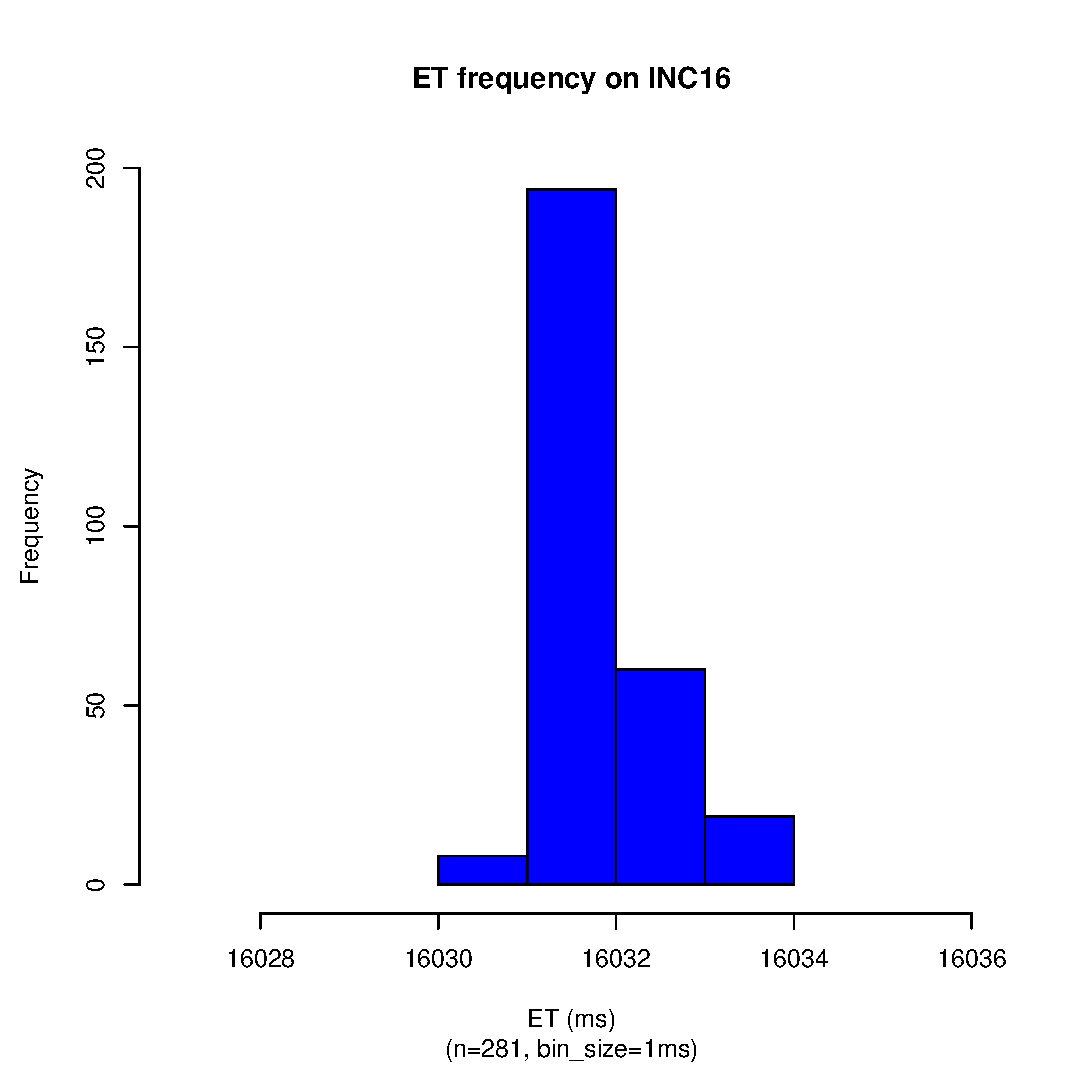
\includegraphics[scale=0.43]{sodb12/16_sec_et_hist_v5.eps}
		\label{fig:s12_inc16_et_hist_v5}
	}
	\subfigure[ET frequency on INC32 on {\tt sodb12}]{
		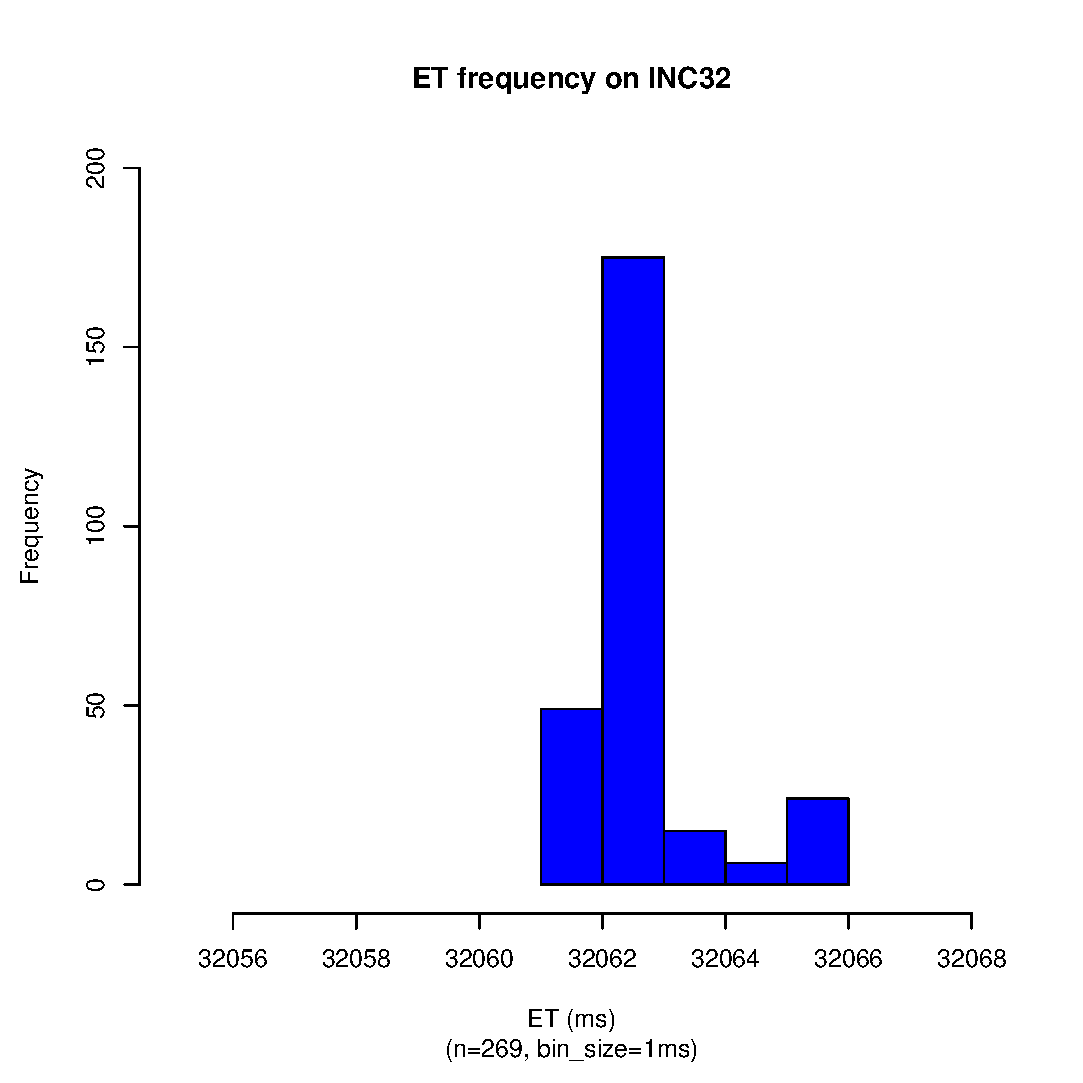
\includegraphics[scale=0.43]{sodb12/32_sec_et_hist_v5.eps}
		\label{fig:s12_inc32_et_hist_v5}
	}
	\subfigure[ET frequency on INC64 on {\tt sodb12}]{
		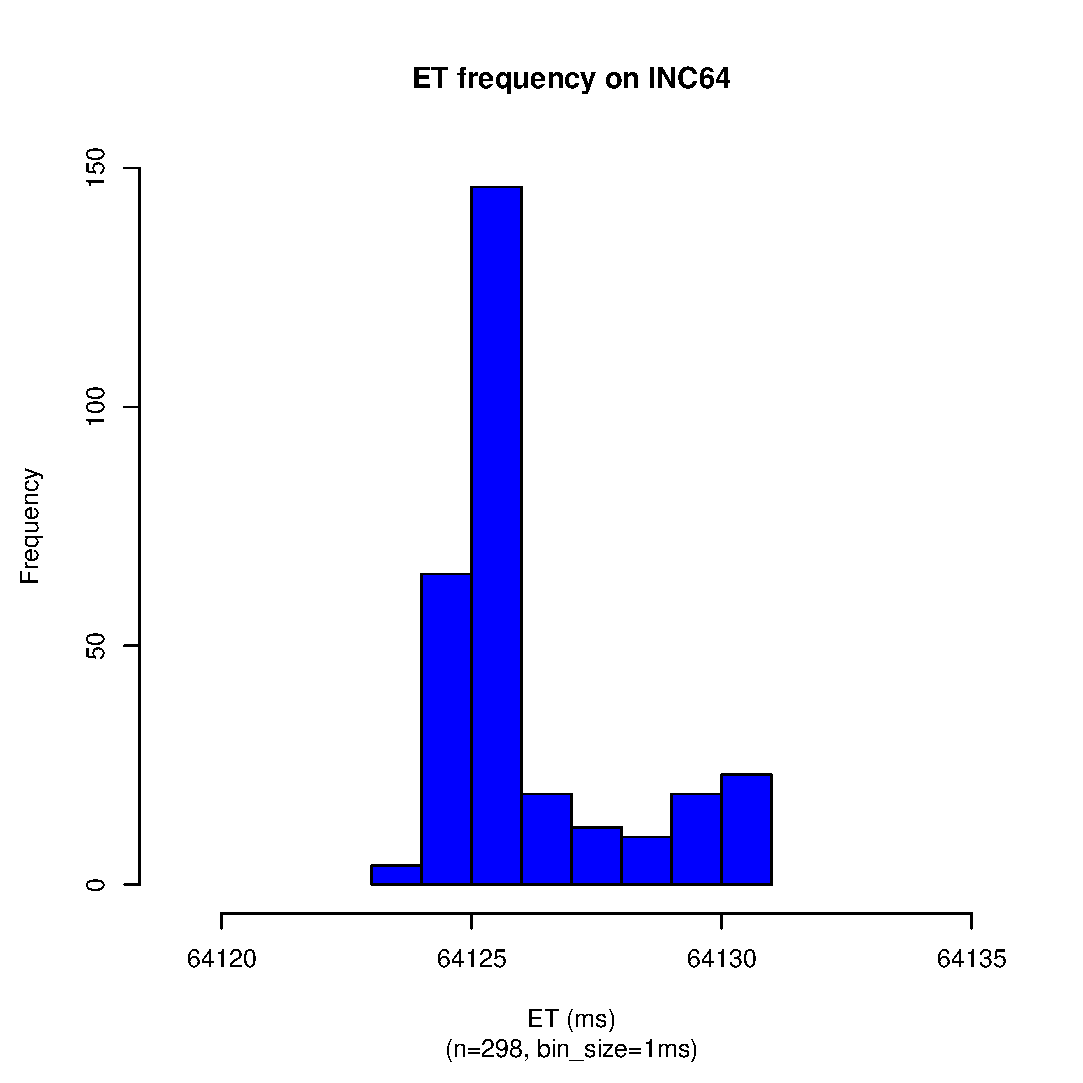
\includegraphics[scale=0.43]{sodb12/64_sec_et_hist_v5.eps}
		\label{fig:s12_inc64_et_hist_v5}
	}
	\subfigure[ET frequency on INC128 on {\tt sodb12}]{
		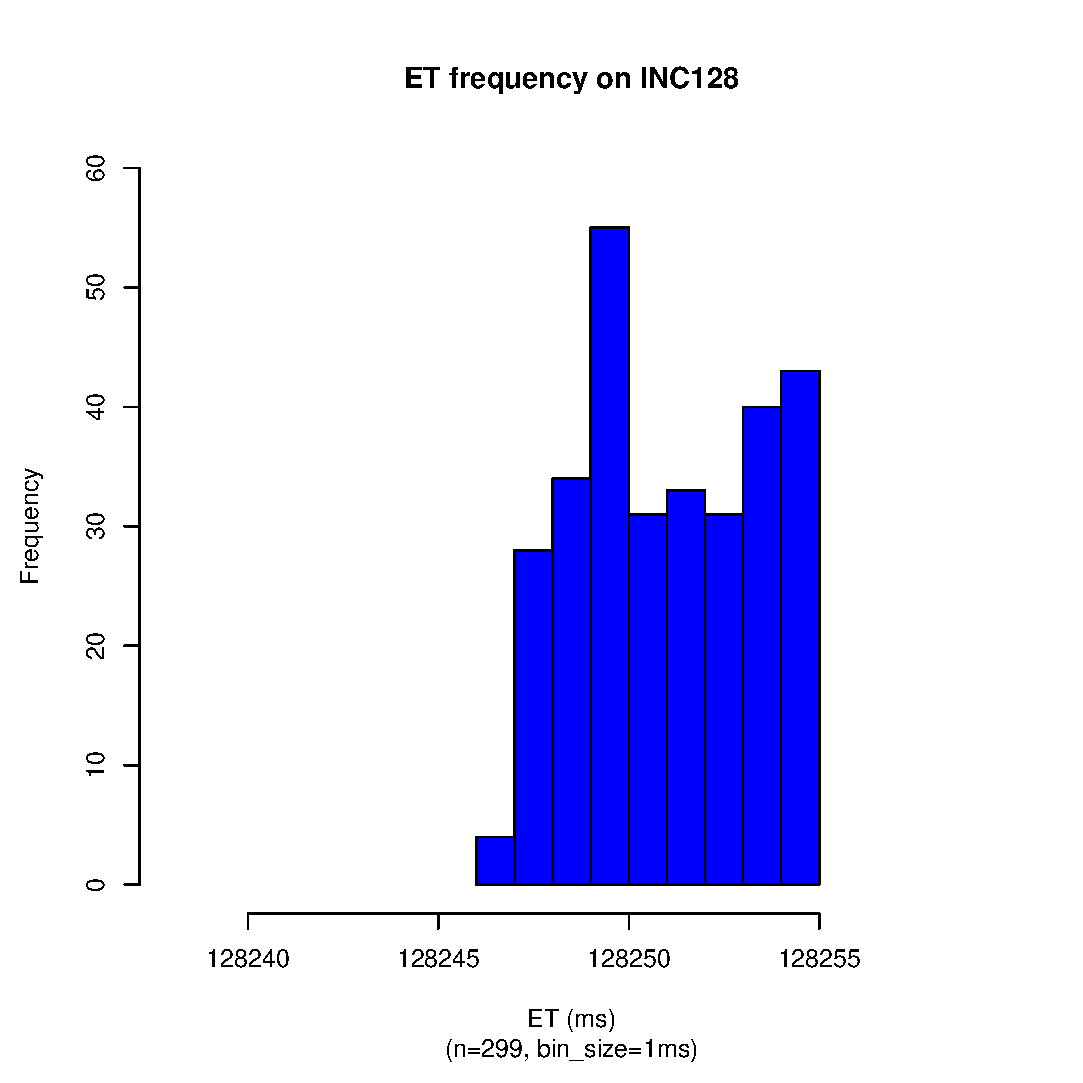
\includegraphics[scale=0.43]{sodb12/128_sec_et_hist_v5.eps}
		\label{fig:s12_inc128_et_hist_v5}
	}
	\caption{ET Histograms of INC16 ... INC128~\label{fig:s12_et_hist2}}
\end{figure}

\newpage

\subsubsection{PT}

\begin{figure}[hp!]
	\centering
	\subfigure[PT frequency on INC1 on {\tt sodb12}]{
		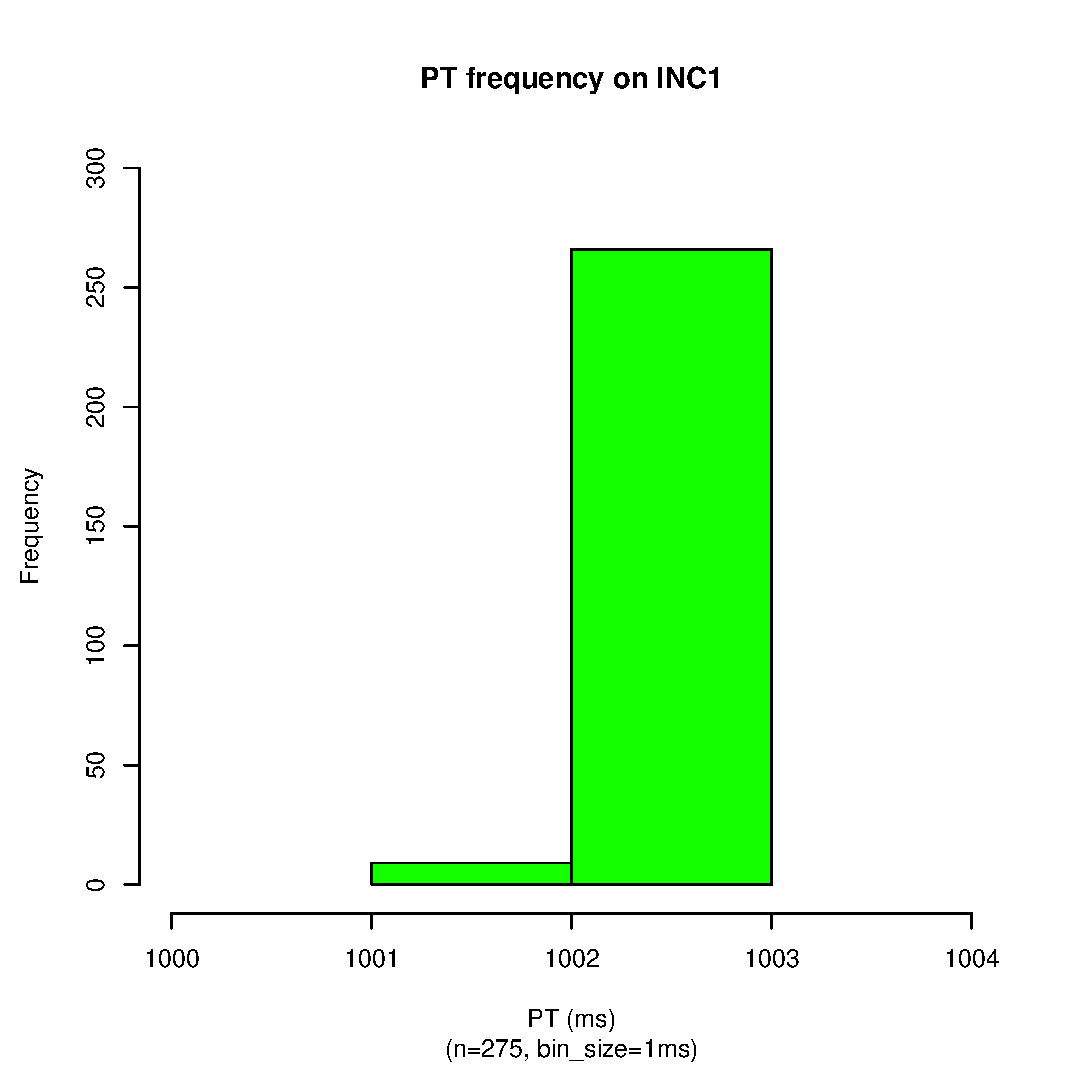
\includegraphics[scale=0.43]{sodb12/1_sec_pt_hist_v5.eps}
		\label{fig:s12_inc1_hist_v5}
	}
	\subfigure[PT frequency on INC2 on {\tt sodb12}]{
		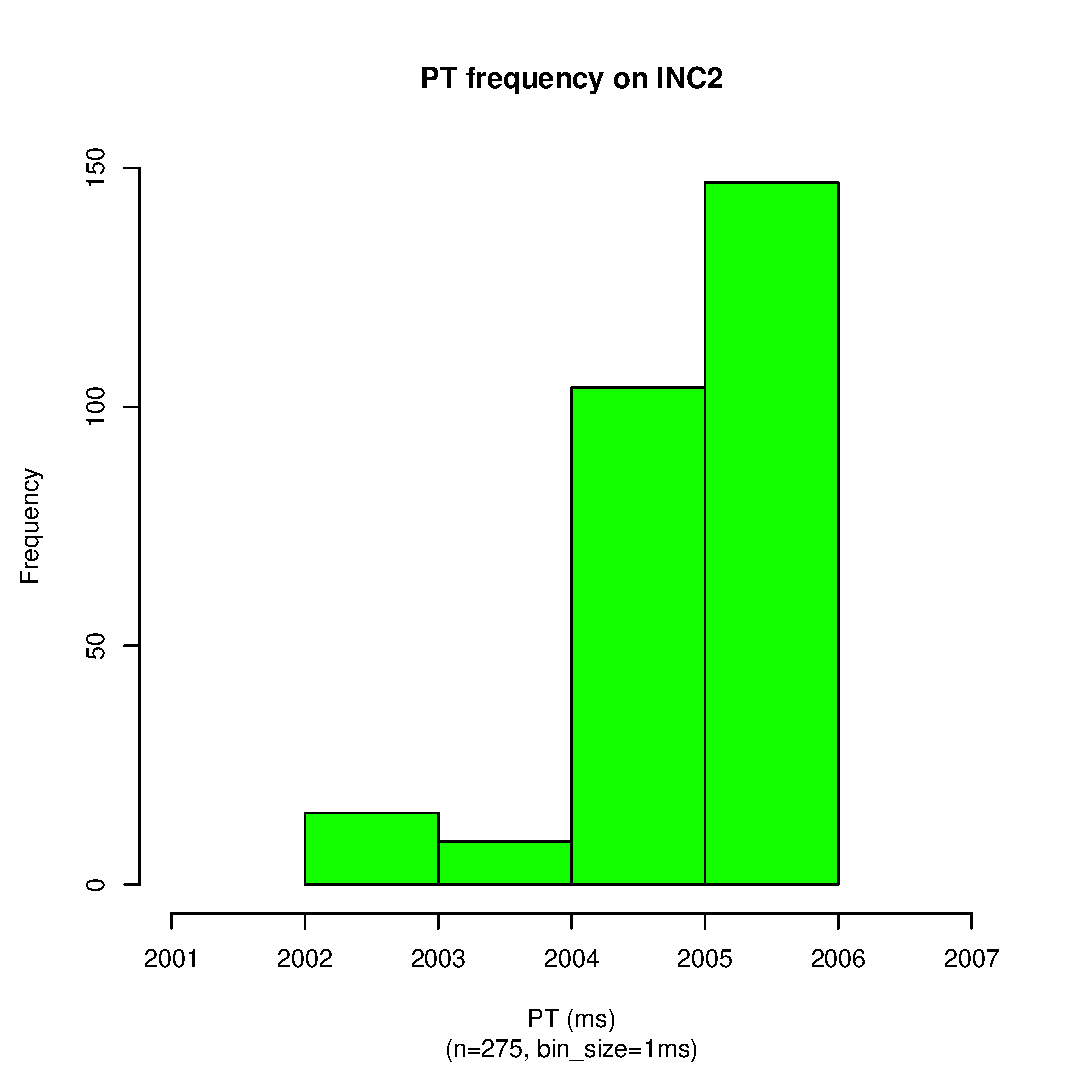
\includegraphics[scale=0.43]{sodb12/2_sec_pt_hist_v5.eps}
		\label{fig:s12_inc2_hist_v5}
	}
	\subfigure[PT frequency on INC4 on {\tt sodb12}]{
		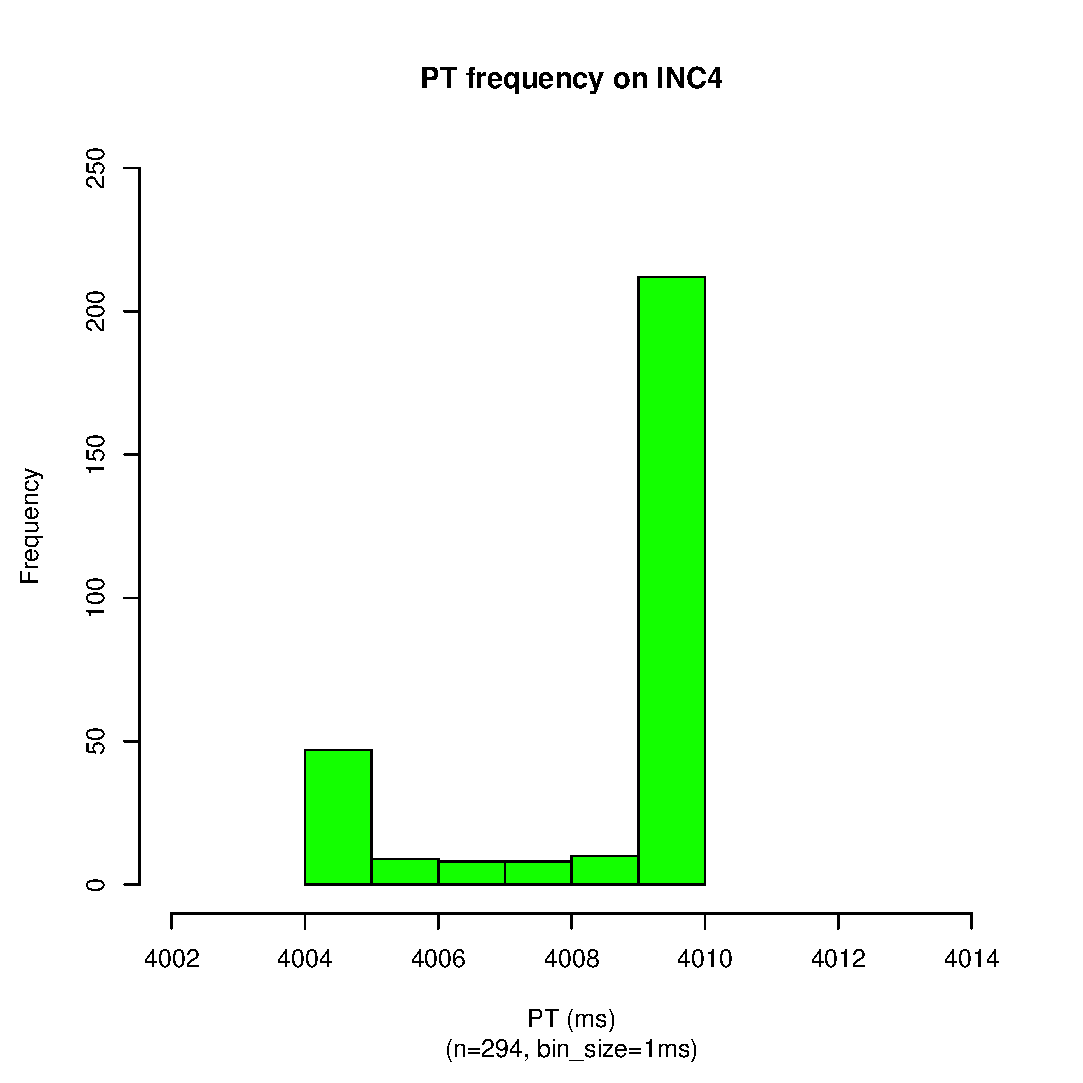
\includegraphics[scale=0.43]{sodb12/4_sec_pt_hist_v5.eps}
		\label{fig:s12_inc4_hist_v5}
	}
	\subfigure[PT frequency on INC8 on {\tt sodb12}]{
		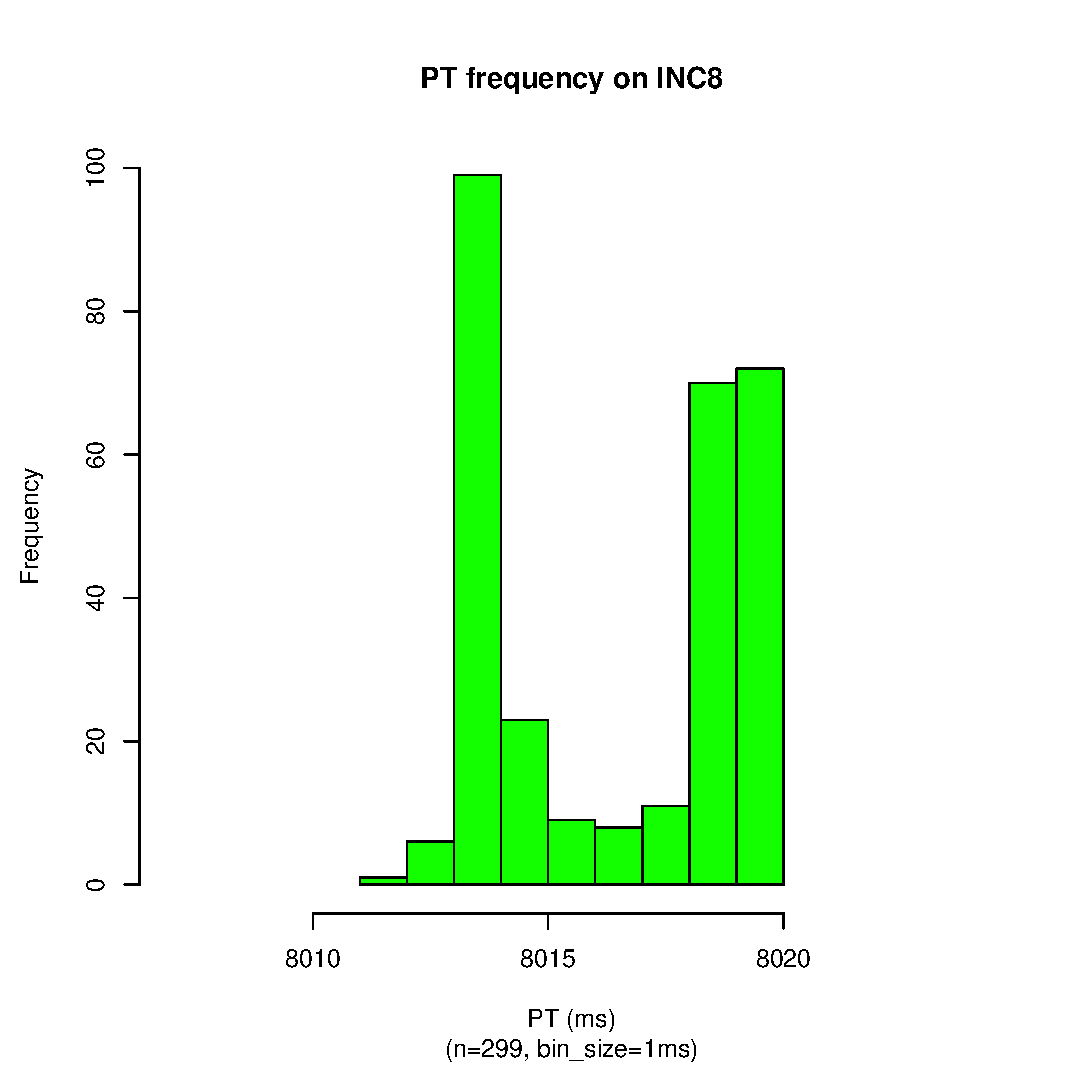
\includegraphics[scale=0.43]{sodb12/8_sec_pt_hist_v5.eps}
		\label{fig:s12_inc8_hist_v5}
	}
	\caption{PT Histograms of INC1 ... INC8~\label{fig:s12_pt_hist1}}
\end{figure}

\begin{figure}[hp!]
	\centering
	\subfigure[PT frequency on INC16 on {\tt sodb12}]{
		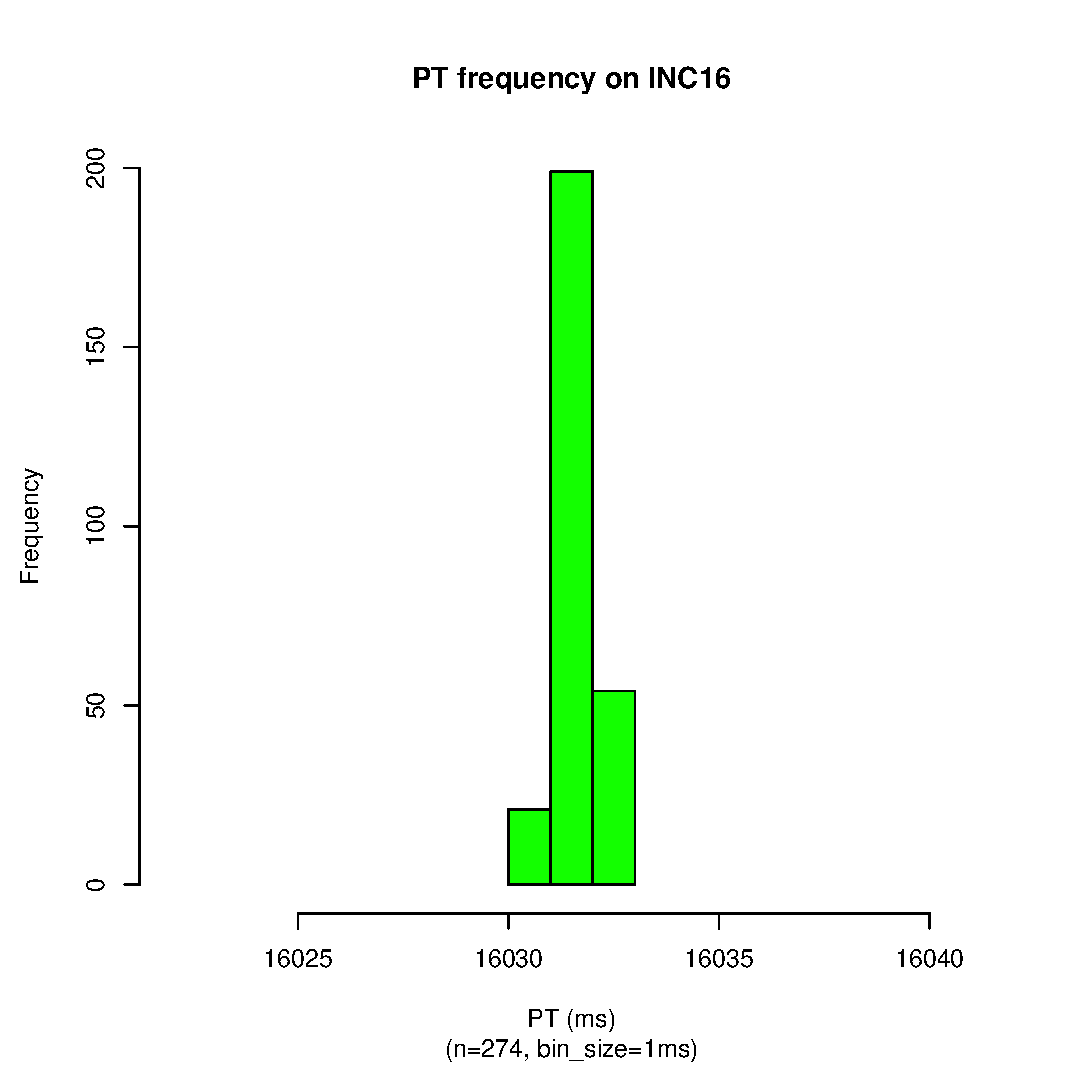
\includegraphics[scale=0.43]{sodb12/16_sec_pt_hist_v5.eps}
		\label{fig:s12_inc16_hist_v5}
	}
	\subfigure[PT frequency on INC32 on {\tt sodb12}]{
		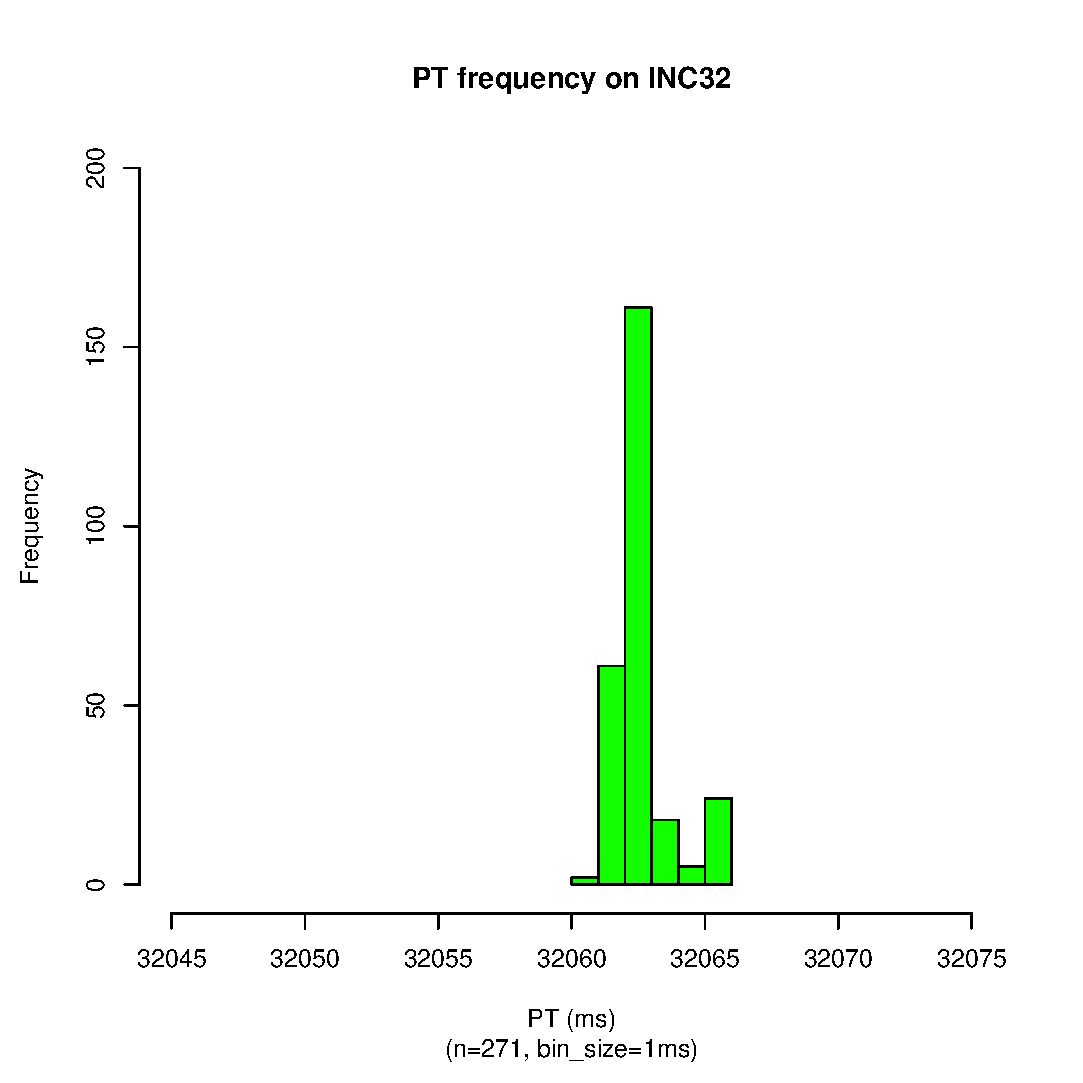
\includegraphics[scale=0.43]{sodb12/32_sec_pt_hist_v5.eps}
		\label{fig:s12_inc32_hist_v5}
	}
	\subfigure[PT frequency on INC64 on {\tt sodb12}]{
		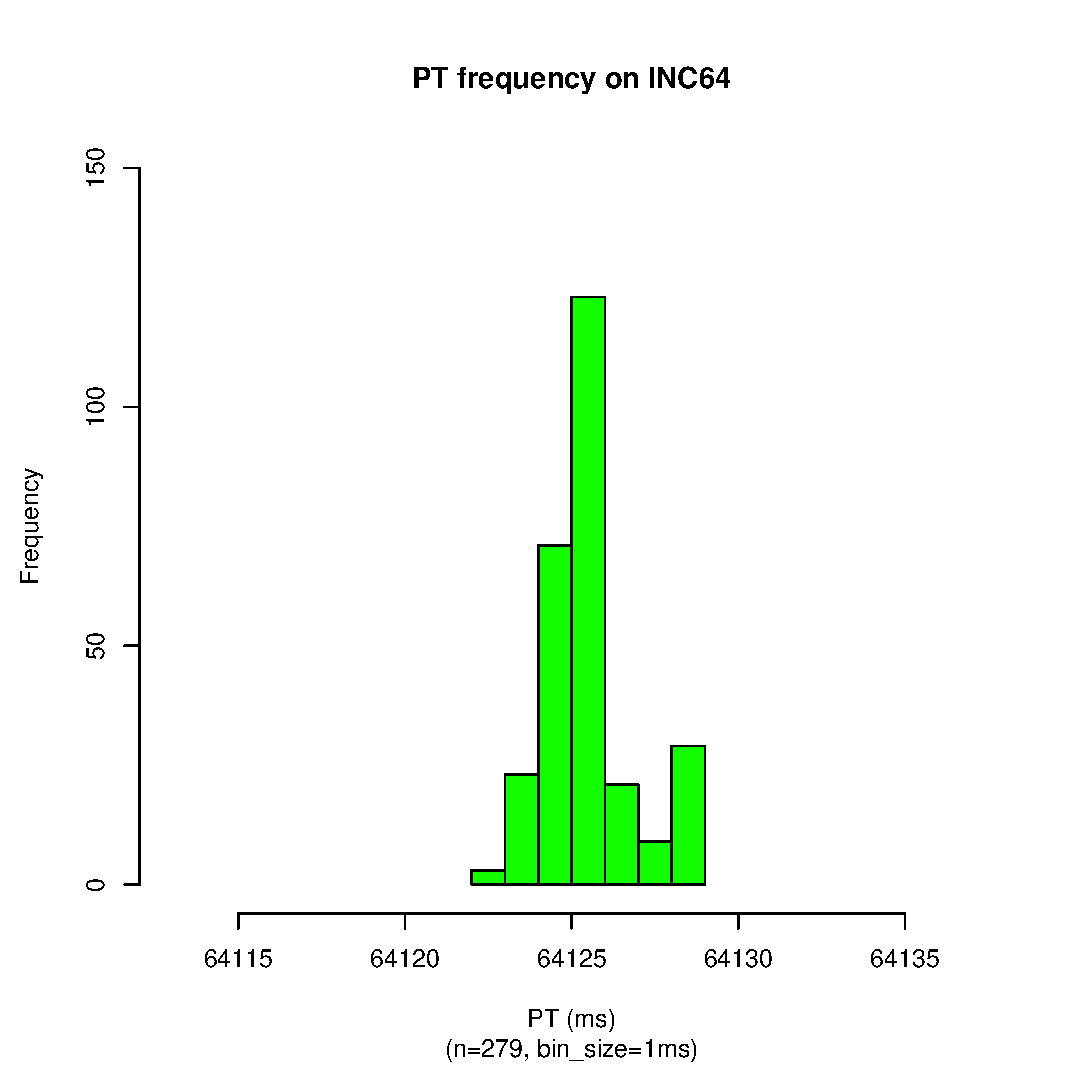
\includegraphics[scale=0.43]{sodb12/64_sec_pt_hist_v5.eps}
		\label{fig:s12_inc64_hist_v5}
	}
	\subfigure[PT frequency on INC128 on {\tt sodb12}]{
		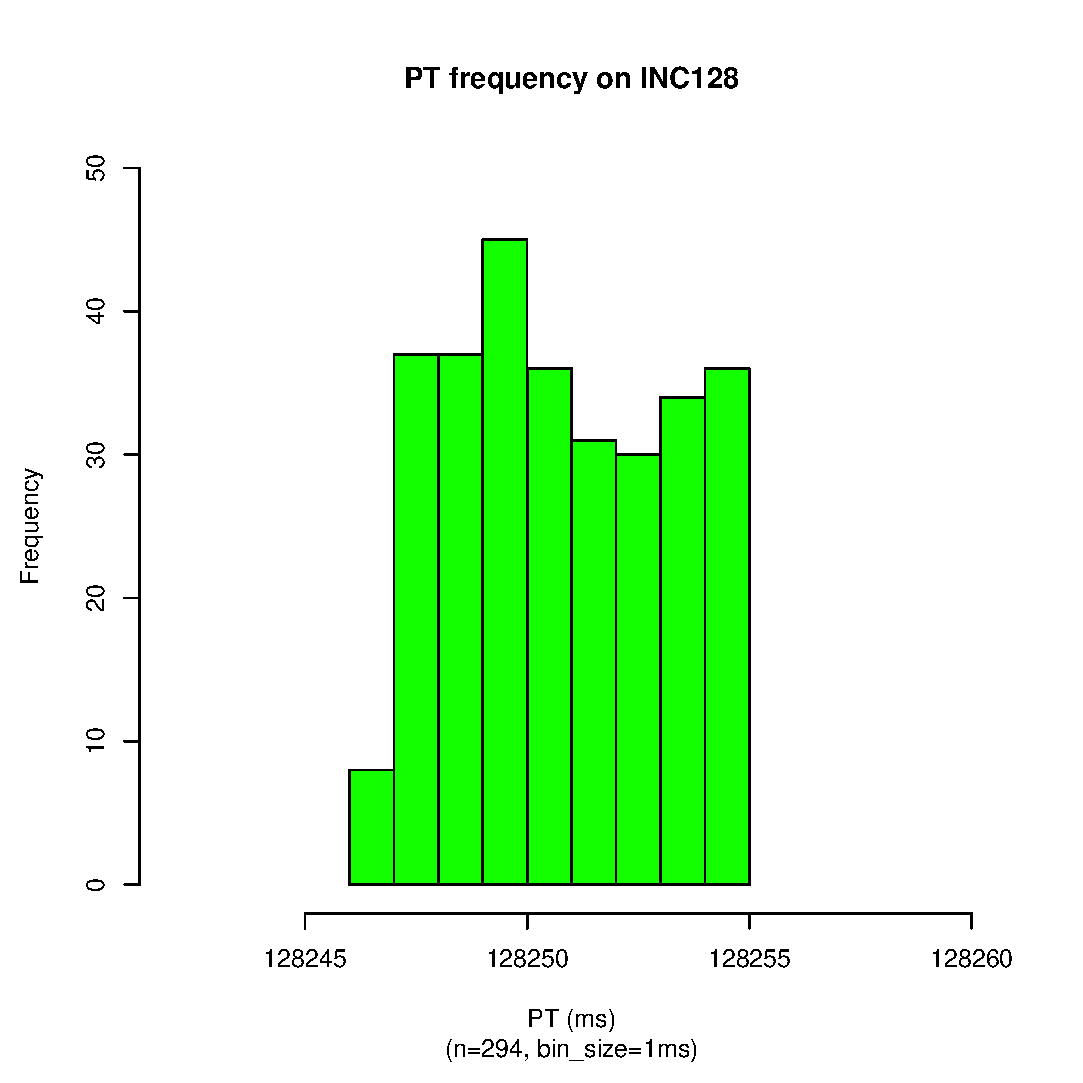
\includegraphics[scale=0.43]{sodb12/128_sec_pt_hist_v5.eps}
		\label{fig:s12_inc128_hist_v5}
	}
	\caption{PT Histograms of INC16 ... INC64~\label{fig:s12_pt_hist2}}
\end{figure}
\newpage

\subsection{{\tt sodb12}~\label{sec:sodb12_hist}} 
This section exhibits histograms on the EMPv5 data obtained on {\tt sodb12}. 
The detailed description of the base data are from Table~\ref{tab:exp_notes}.

\subsubsection{ET}

\begin{figure}[hp!]
	\centering
	\subfigure[ET frequency on INC1 on {\tt sodb12}]{
		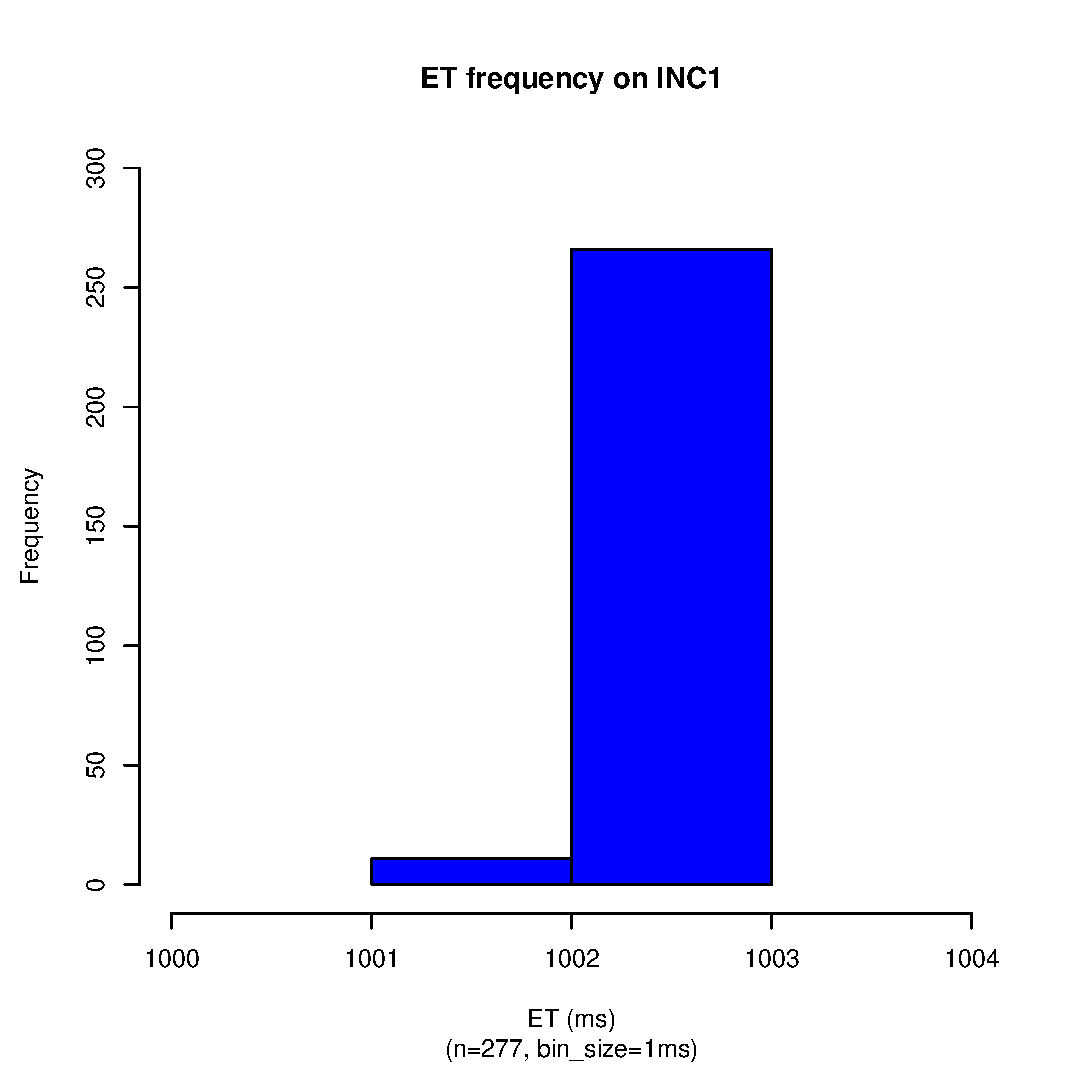
\includegraphics[scale=0.43]{sodb12/1_sec_et_hist_v5.eps}
		\label{fig:s12_inc1_et_hist_v5}
	}
	\subfigure[ET frequency on INC2 on {\tt sodb12}]{
		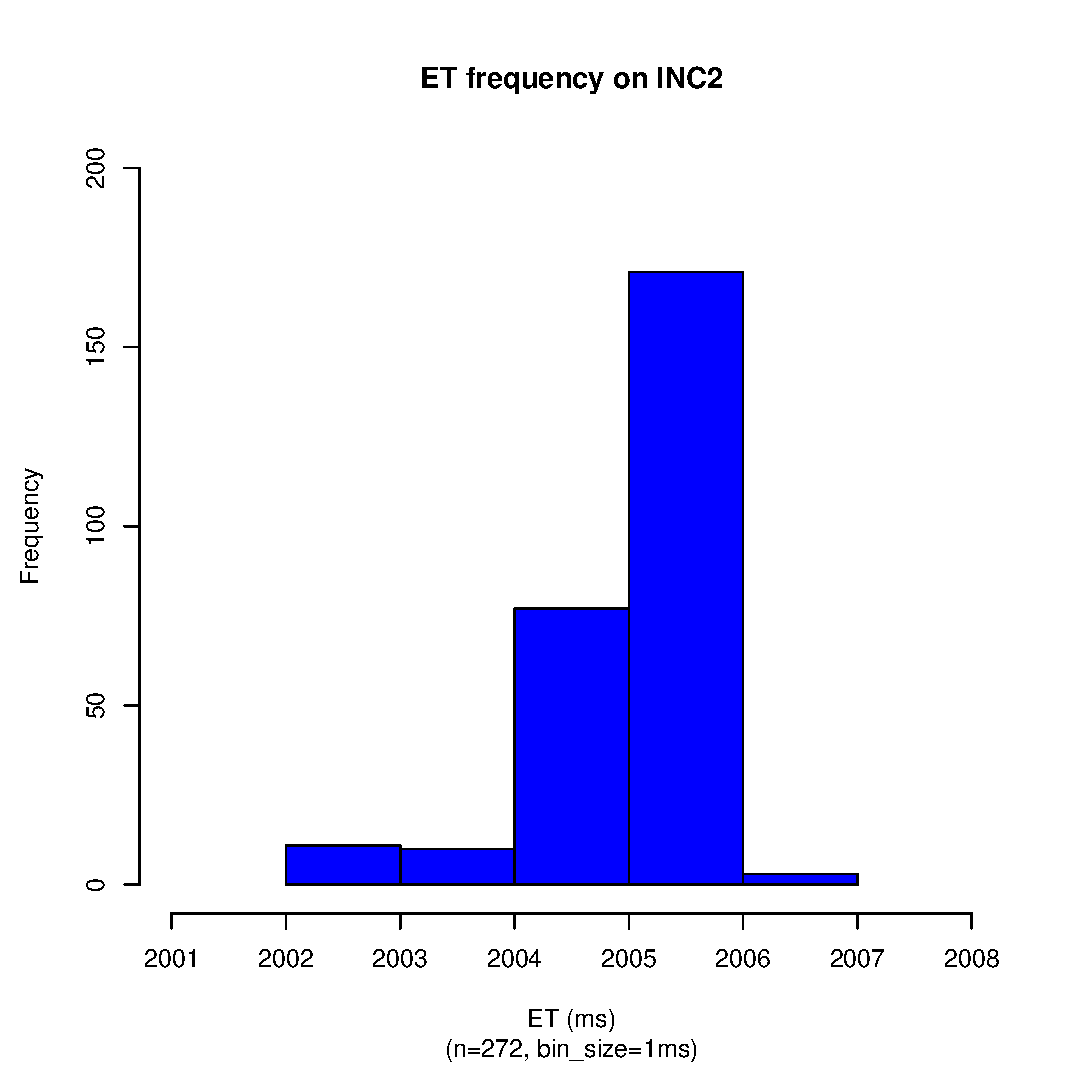
\includegraphics[scale=0.43]{sodb12/2_sec_et_hist_v5.eps}
		\label{fig:s12_inc2_et_hist_v5}
	}
	\subfigure[ET frequency on INC4 on {\tt sodb12}]{
		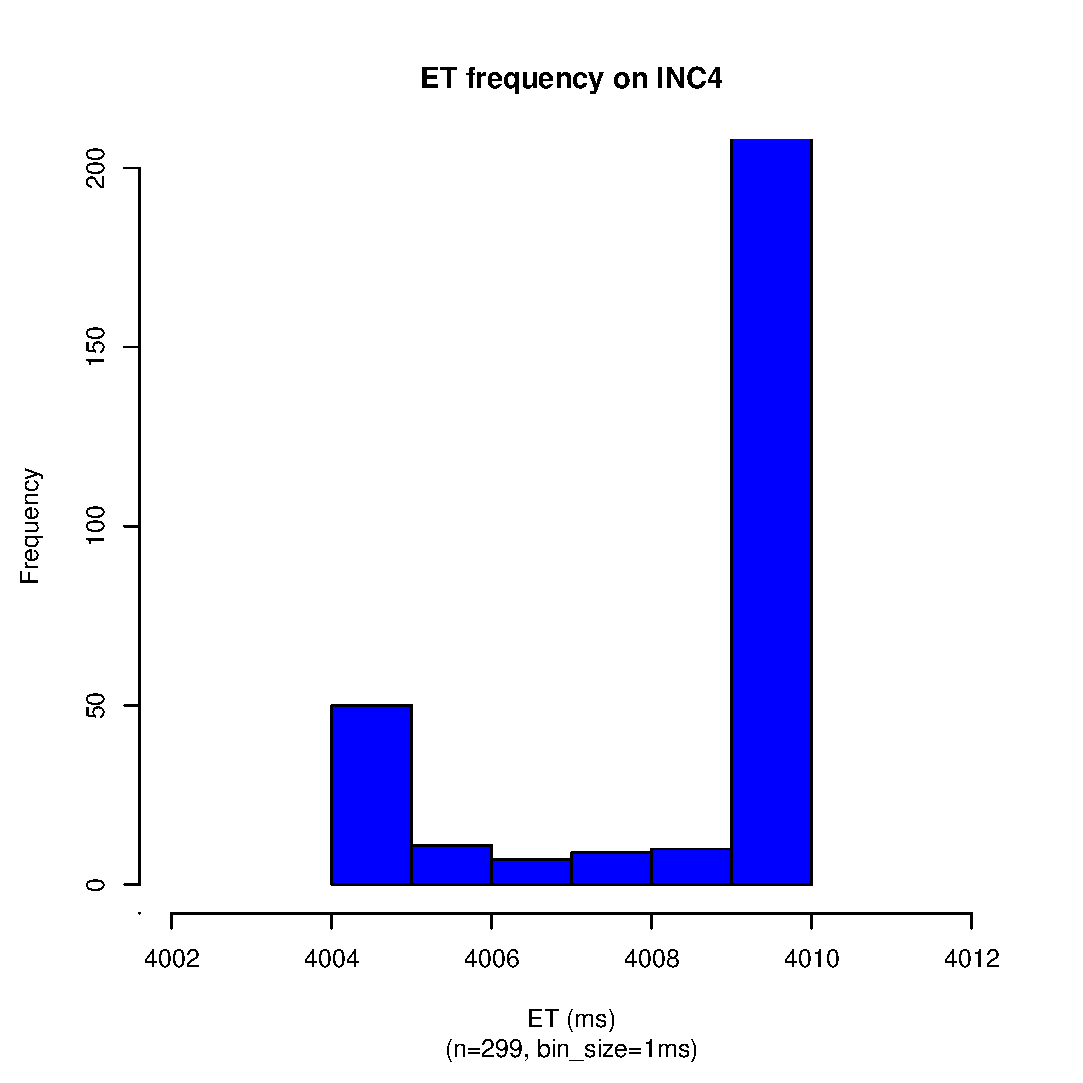
\includegraphics[scale=0.43]{sodb12/4_sec_et_hist_v5.eps}
		\label{fig:s12_inc4_et_hist_v5}
	}
	\subfigure[ET frequency on INC8 on {\tt sodb12}]{
		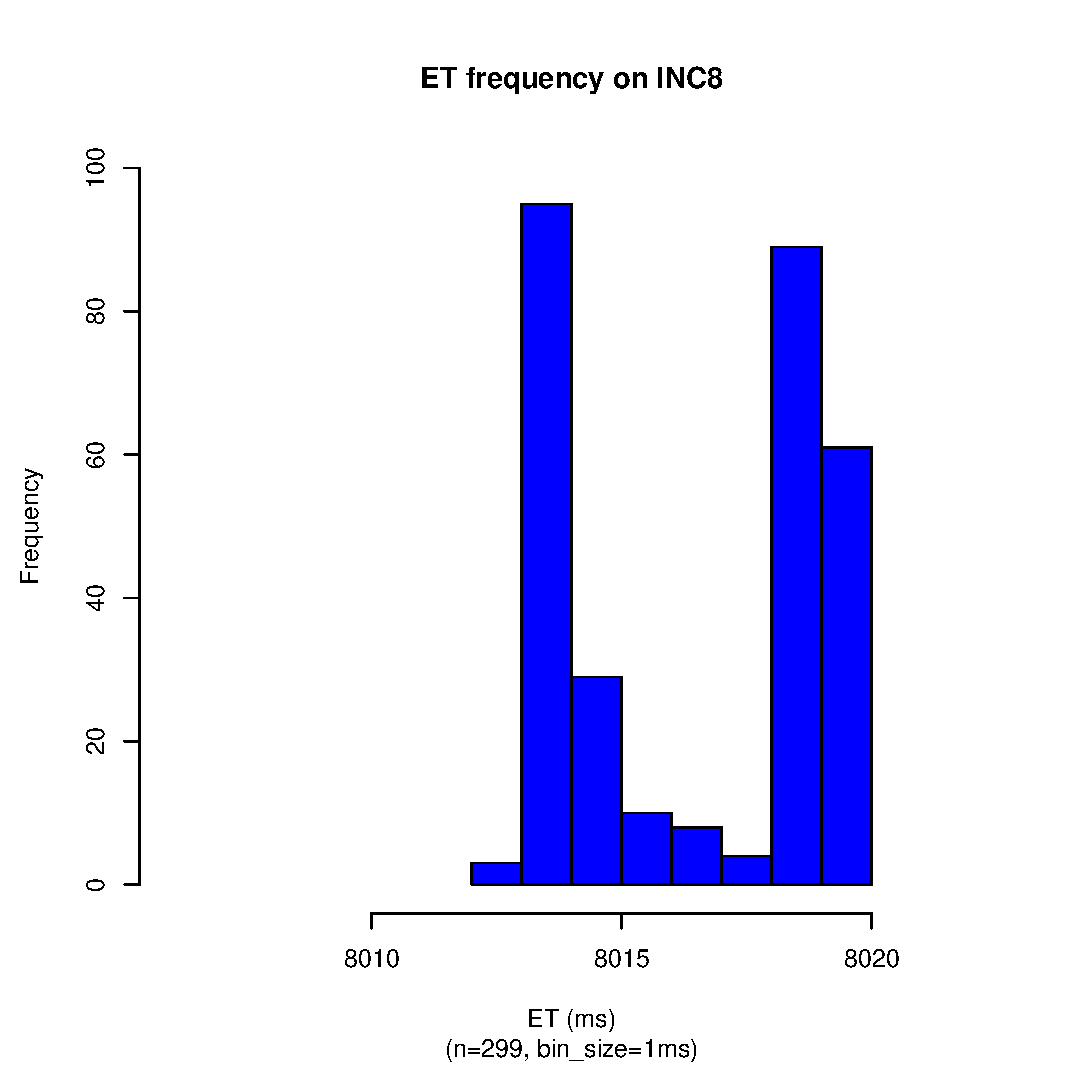
\includegraphics[scale=0.43]{sodb12/8_sec_et_hist_v5.eps}
		\label{fig:s12_inc8_et_hist_v5}
	}
	\caption{ET Histograms of INC1 ... INC8~\label{fig:s12_et_hist1}}
\end{figure}

\begin{figure}[hp!]
	\centering
	\subfigure[ET frequency on INC16 on {\tt sodb12}]{
		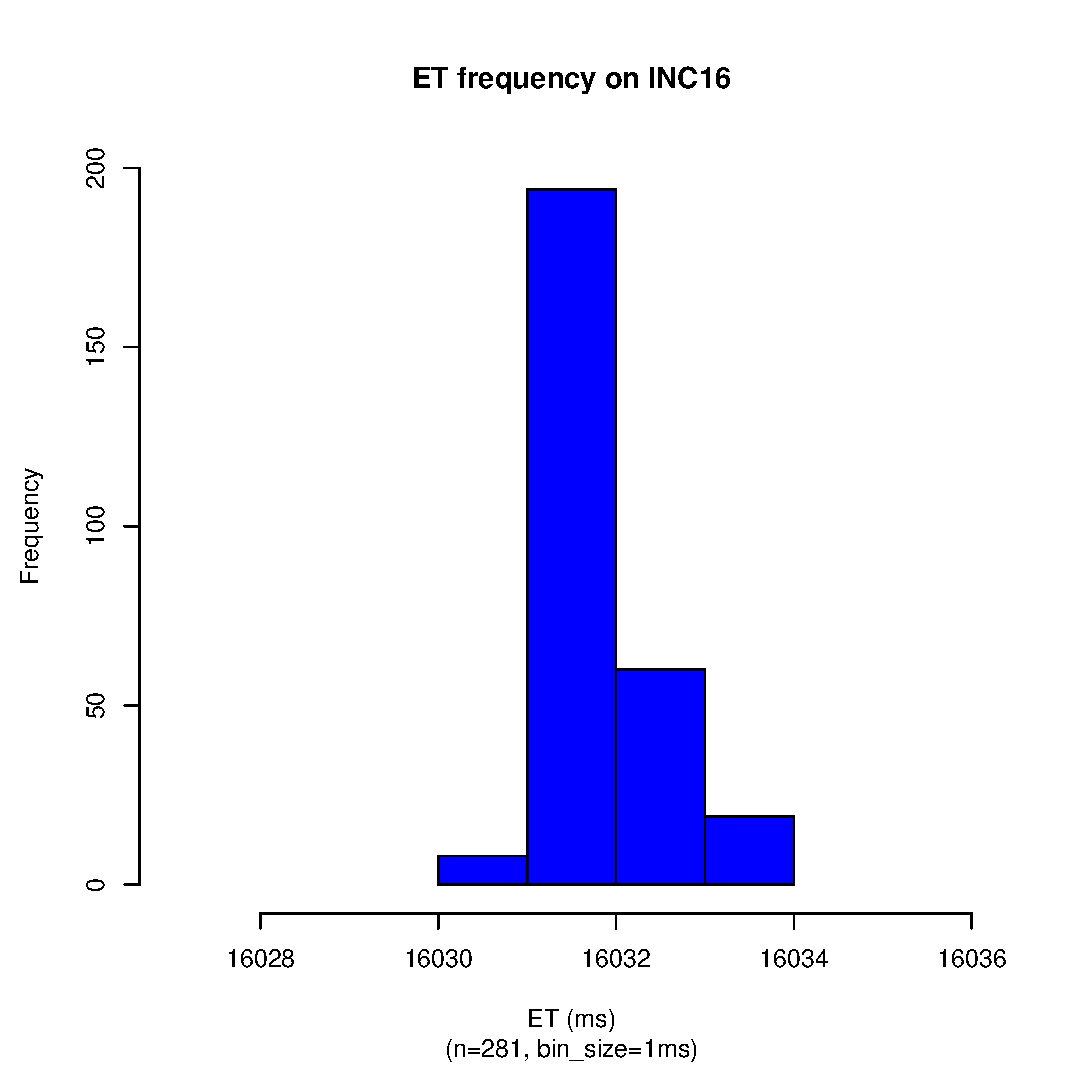
\includegraphics[scale=0.43]{sodb12/16_sec_et_hist_v5.eps}
		\label{fig:s12_inc16_et_hist_v5}
	}
	\subfigure[ET frequency on INC32 on {\tt sodb12}]{
		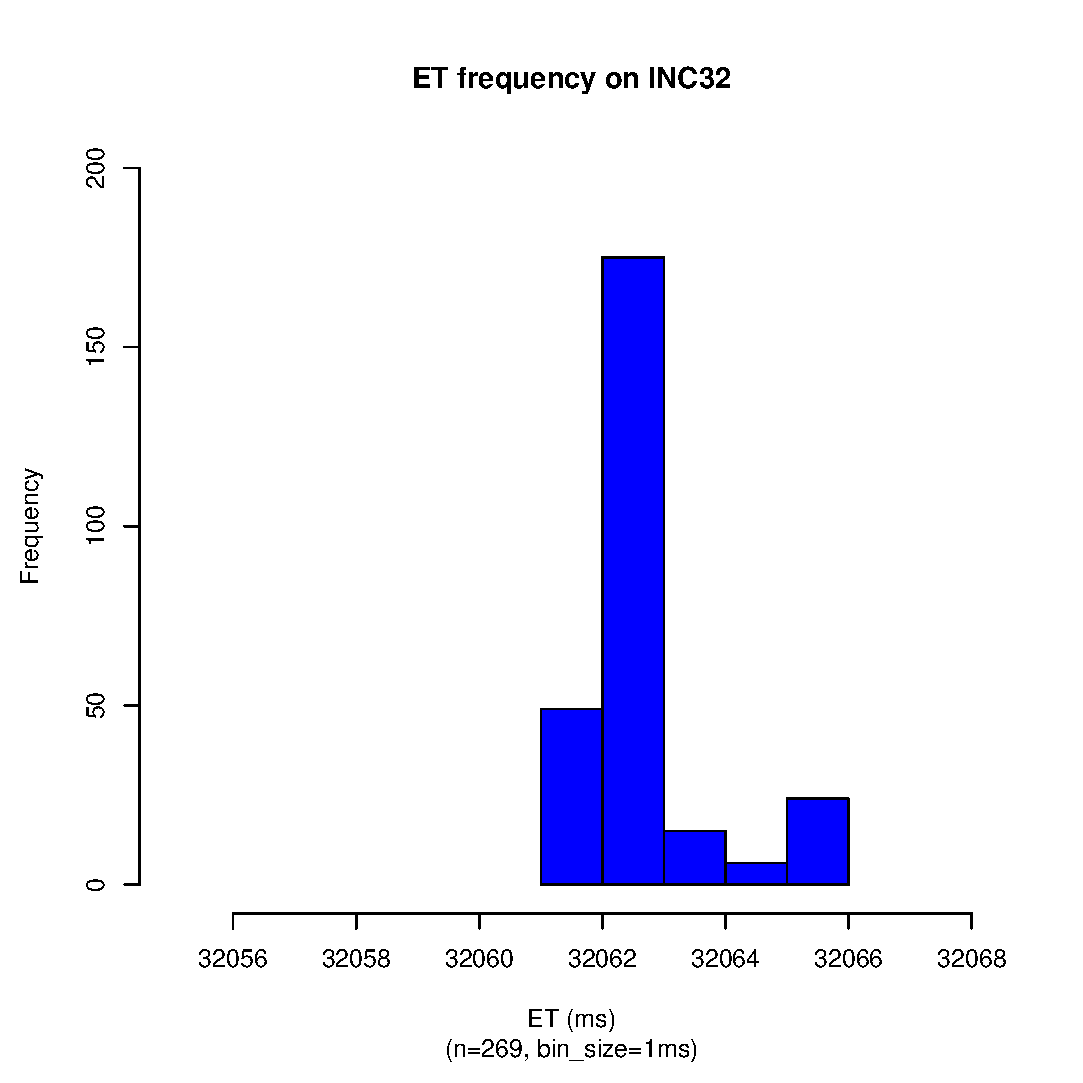
\includegraphics[scale=0.43]{sodb12/32_sec_et_hist_v5.eps}
		\label{fig:s12_inc32_et_hist_v5}
	}
	\subfigure[ET frequency on INC64 on {\tt sodb12}]{
		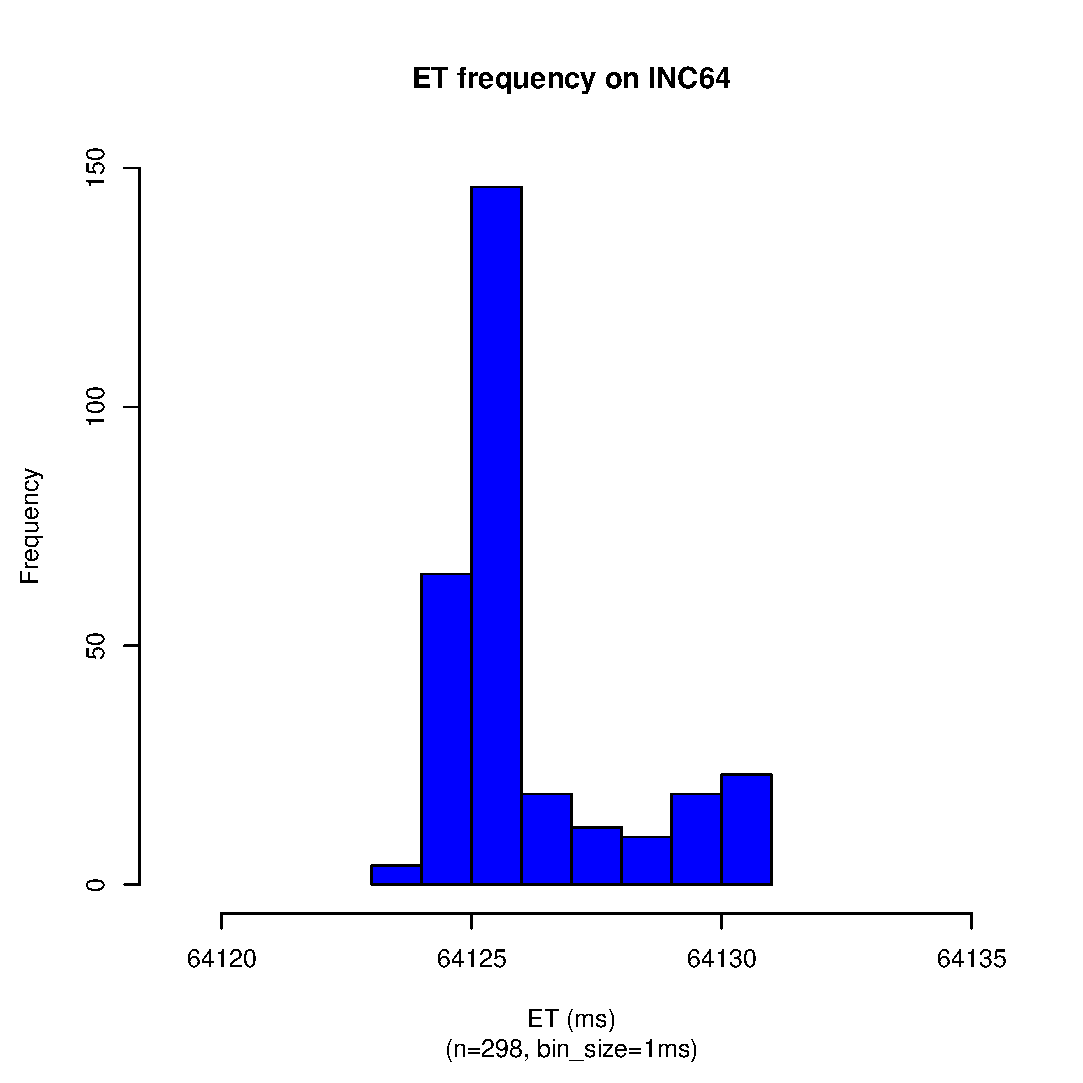
\includegraphics[scale=0.43]{sodb12/64_sec_et_hist_v5.eps}
		\label{fig:s12_inc64_et_hist_v5}
	}
	\subfigure[ET frequency on INC128 on {\tt sodb12}]{
		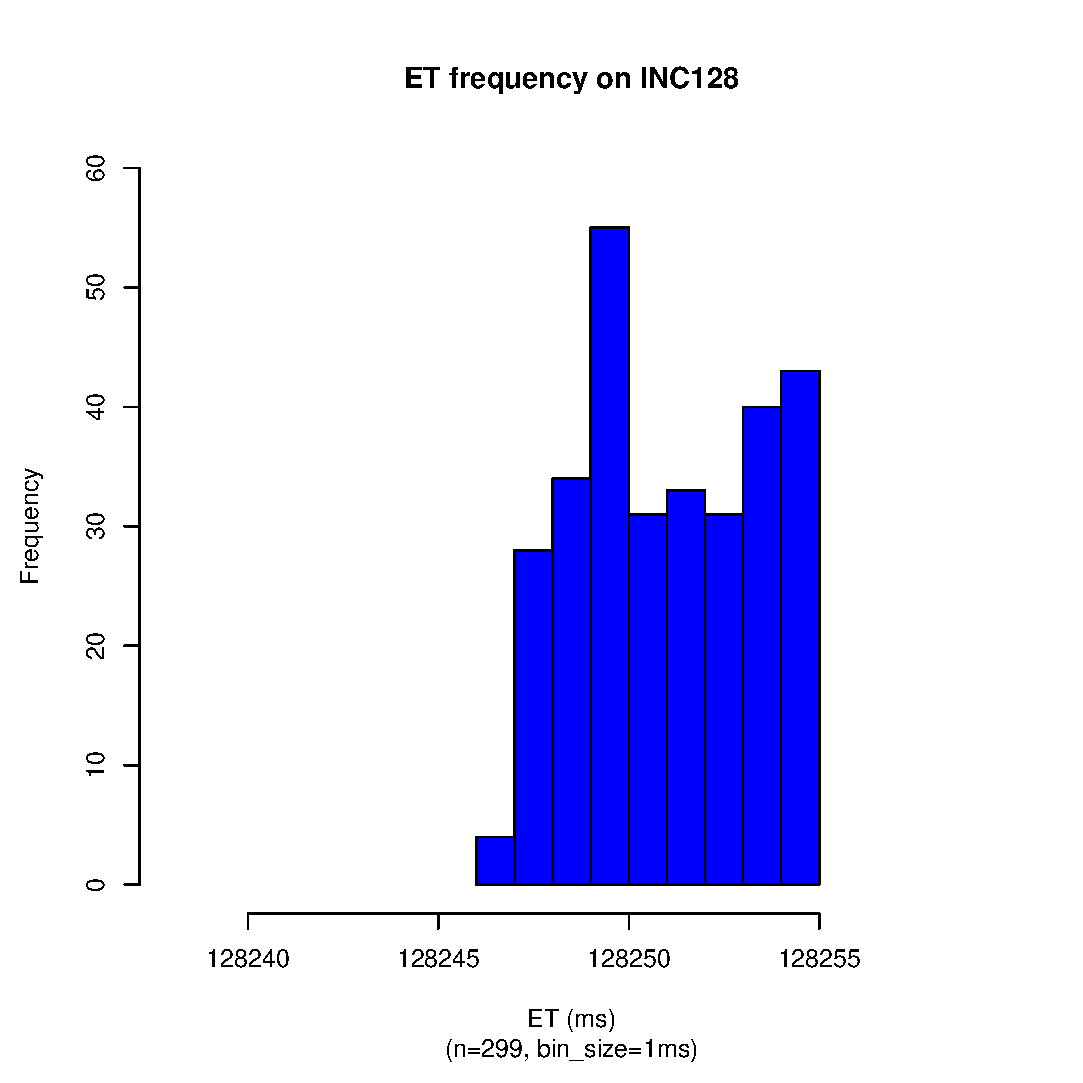
\includegraphics[scale=0.43]{sodb12/128_sec_et_hist_v5.eps}
		\label{fig:s12_inc128_et_hist_v5}
	}
	\caption{ET Histograms of INC16 ... INC128~\label{fig:s12_et_hist2}}
\end{figure}

\newpage

\subsubsection{PT}

\begin{figure}[hp!]
	\centering
	\subfigure[PT frequency on INC1 on {\tt sodb12}]{
		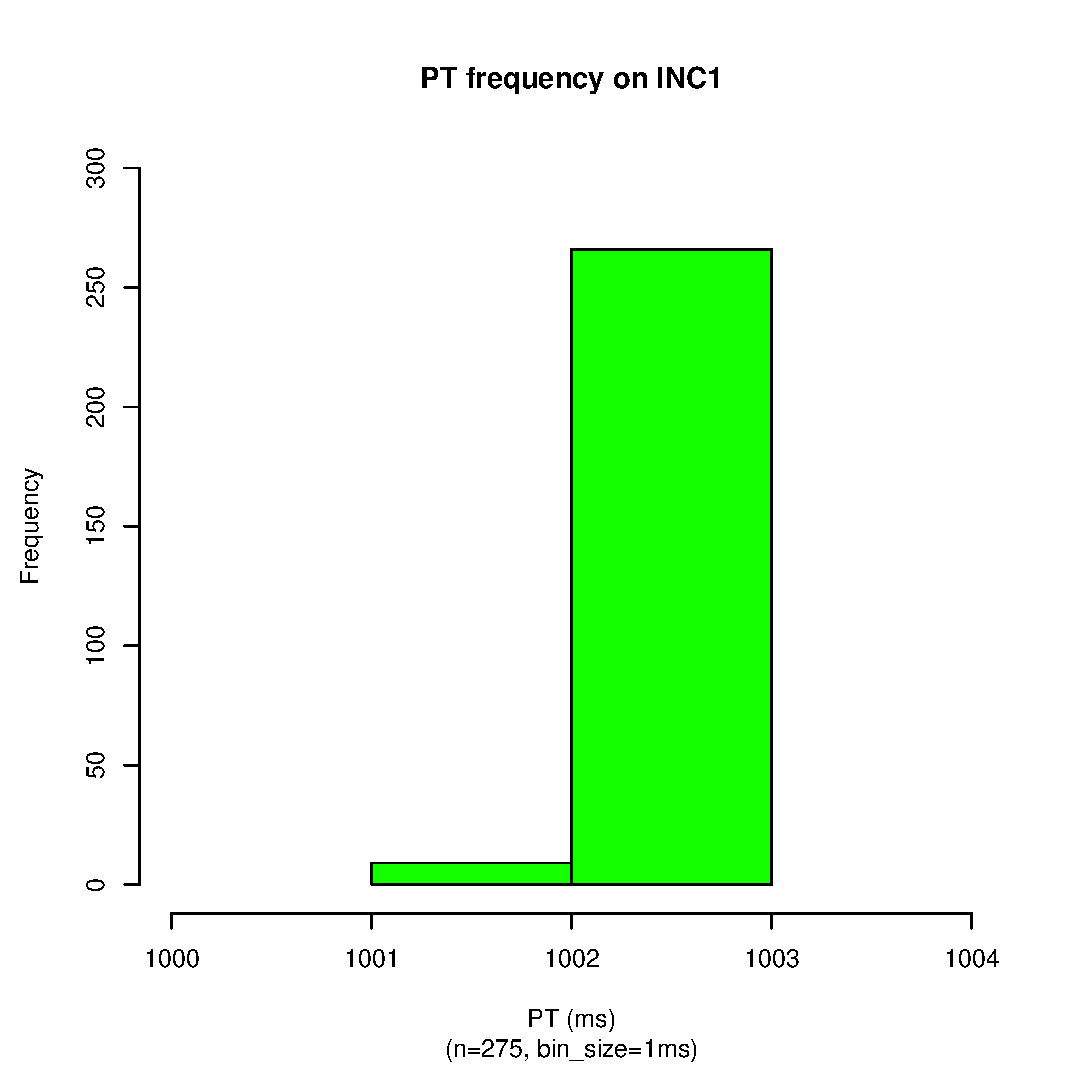
\includegraphics[scale=0.43]{sodb12/1_sec_pt_hist_v5.eps}
		\label{fig:s12_inc1_hist_v5}
	}
	\subfigure[PT frequency on INC2 on {\tt sodb12}]{
		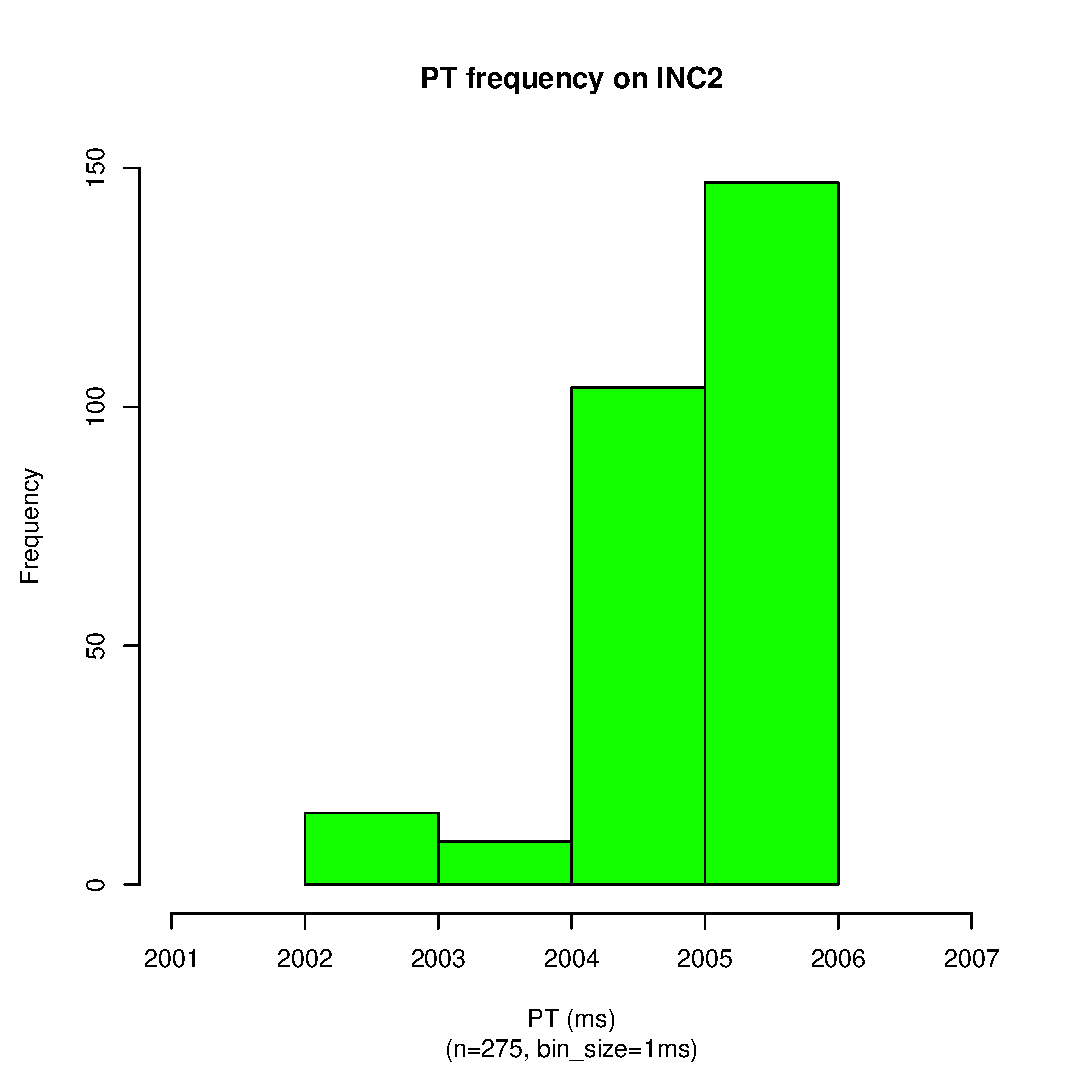
\includegraphics[scale=0.43]{sodb12/2_sec_pt_hist_v5.eps}
		\label{fig:s12_inc2_hist_v5}
	}
	\subfigure[PT frequency on INC4 on {\tt sodb12}]{
		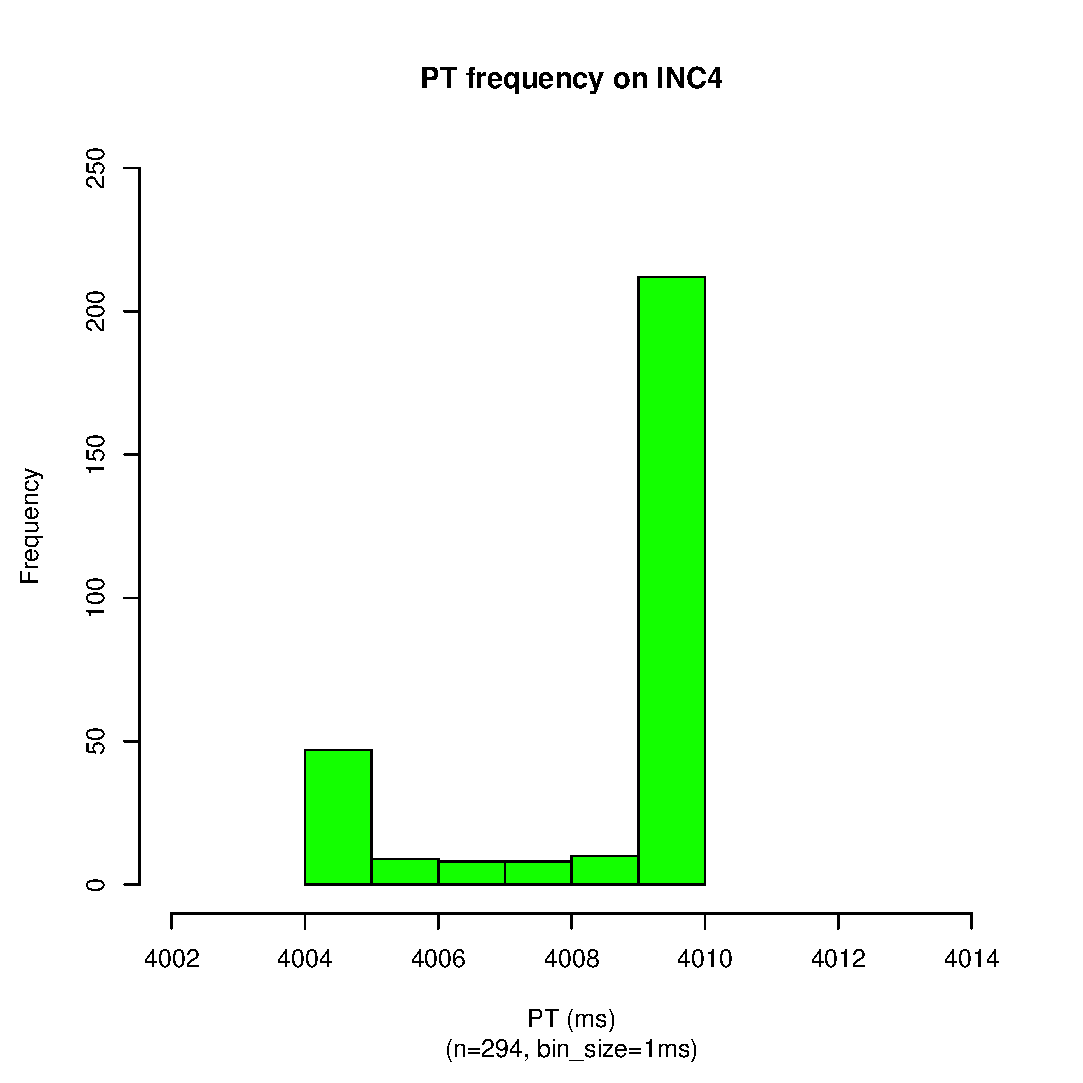
\includegraphics[scale=0.43]{sodb12/4_sec_pt_hist_v5.eps}
		\label{fig:s12_inc4_hist_v5}
	}
	\subfigure[PT frequency on INC8 on {\tt sodb12}]{
		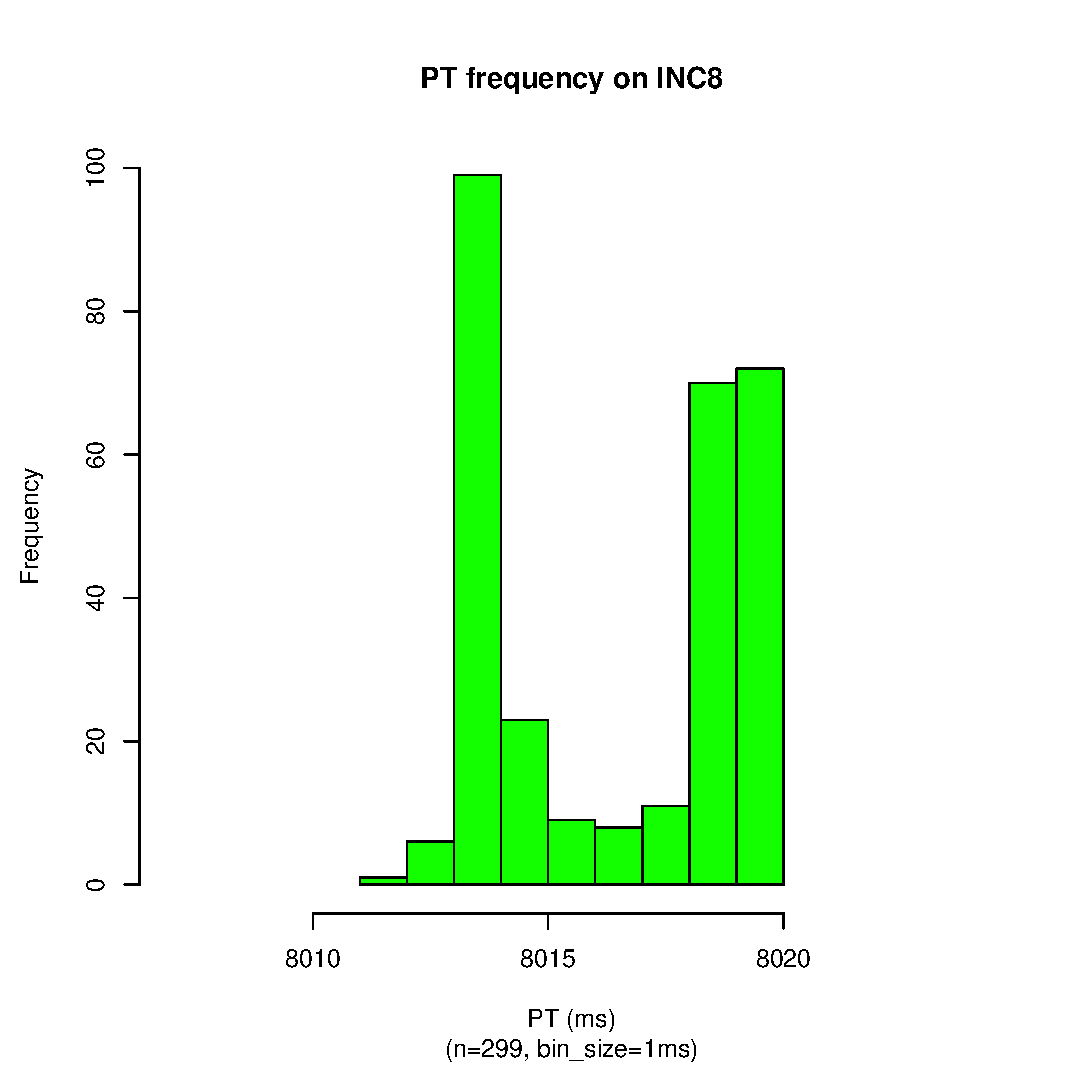
\includegraphics[scale=0.43]{sodb12/8_sec_pt_hist_v5.eps}
		\label{fig:s12_inc8_hist_v5}
	}
	\caption{PT Histograms of INC1 ... INC8~\label{fig:s12_pt_hist1}}
\end{figure}

\begin{figure}[hp!]
	\centering
	\subfigure[PT frequency on INC16 on {\tt sodb12}]{
		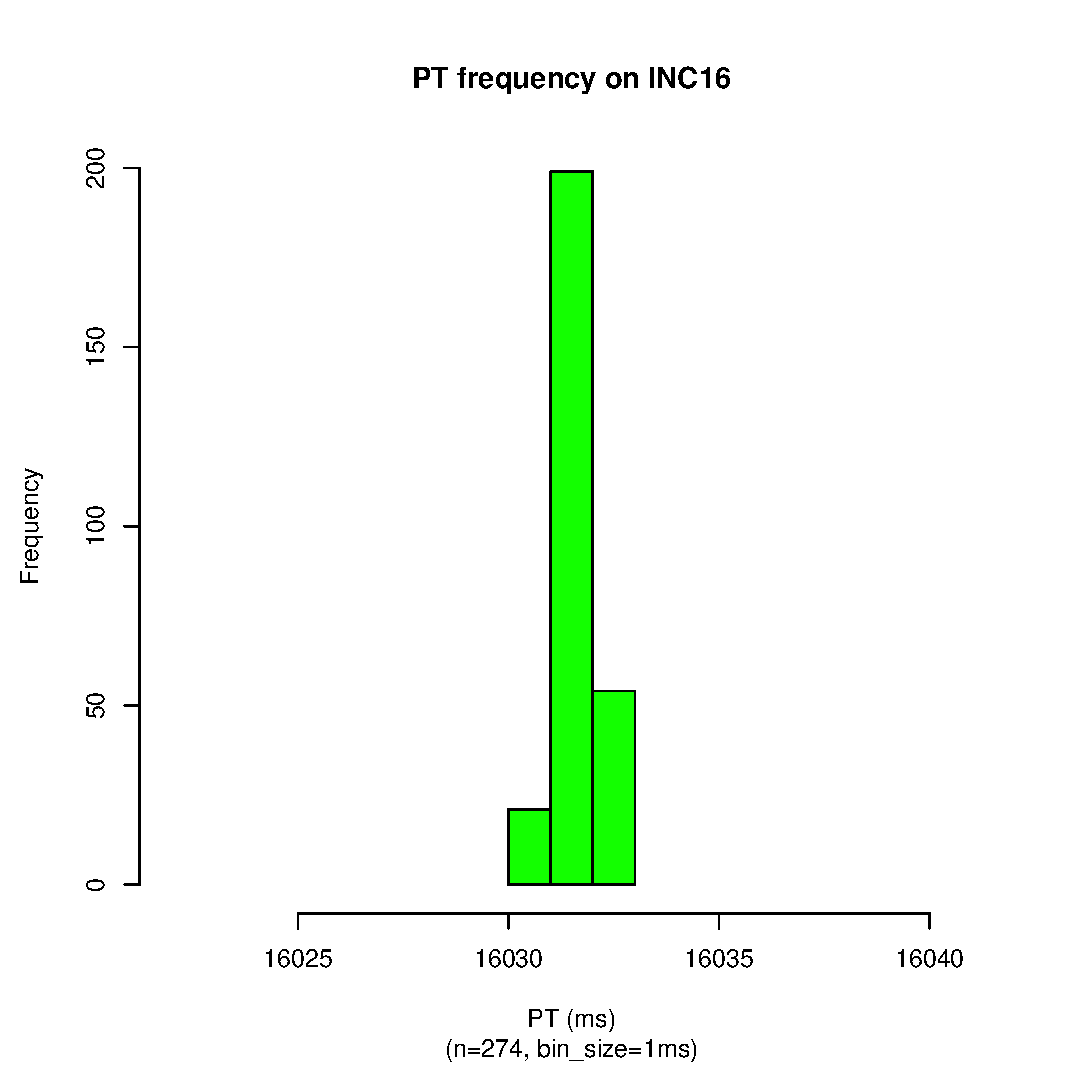
\includegraphics[scale=0.43]{sodb12/16_sec_pt_hist_v5.eps}
		\label{fig:s12_inc16_hist_v5}
	}
	\subfigure[PT frequency on INC32 on {\tt sodb12}]{
		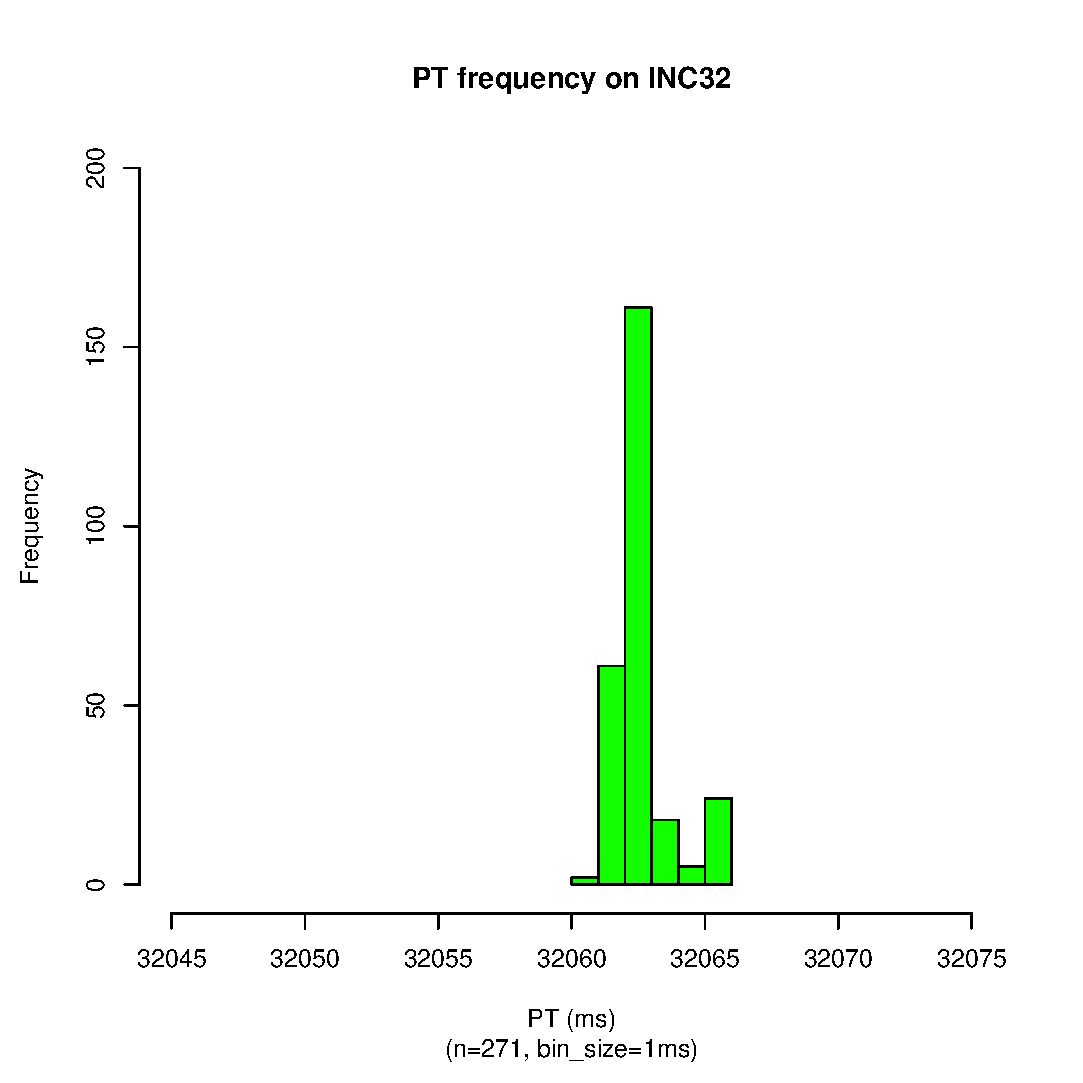
\includegraphics[scale=0.43]{sodb12/32_sec_pt_hist_v5.eps}
		\label{fig:s12_inc32_hist_v5}
	}
	\subfigure[PT frequency on INC64 on {\tt sodb12}]{
		\includegraphics[scale=0.43]{sodb12/64_sec_pt_hist_v5.eps}
		\label{fig:s12_inc64_hist_v5}
	}
	\subfigure[PT frequency on INC128 on {\tt sodb12}]{
		\includegraphics[scale=0.43]{sodb12/128_sec_pt_hist_v5.eps}
		\label{fig:s12_inc128_hist_v5}
	}
	\caption{PT Histograms of INC16 ... INC64~\label{fig:s12_pt_hist2}}
\end{figure}
\newpage

\subsection{{\tt sodb12}~\label{sec:sodb12_hist}} 
This section exhibits histograms on the EMPv5 data obtained on {\tt sodb12}. 
The detailed description of the base data are from Table~\ref{tab:exp_notes}.

\subsubsection{ET}

\begin{figure}[hp!]
	\centering
	\subfigure[ET frequency on INC1 on {\tt sodb12}]{
		\includegraphics[scale=0.43]{sodb12/1_sec_et_hist_v5.eps}
		\label{fig:s12_inc1_et_hist_v5}
	}
	\subfigure[ET frequency on INC2 on {\tt sodb12}]{
		\includegraphics[scale=0.43]{sodb12/2_sec_et_hist_v5.eps}
		\label{fig:s12_inc2_et_hist_v5}
	}
	\subfigure[ET frequency on INC4 on {\tt sodb12}]{
		\includegraphics[scale=0.43]{sodb12/4_sec_et_hist_v5.eps}
		\label{fig:s12_inc4_et_hist_v5}
	}
	\subfigure[ET frequency on INC8 on {\tt sodb12}]{
		\includegraphics[scale=0.43]{sodb12/8_sec_et_hist_v5.eps}
		\label{fig:s12_inc8_et_hist_v5}
	}
	\caption{ET Histograms of INC1 ... INC8~\label{fig:s12_et_hist1}}
\end{figure}

\begin{figure}[hp!]
	\centering
	\subfigure[ET frequency on INC16 on {\tt sodb12}]{
		\includegraphics[scale=0.43]{sodb12/16_sec_et_hist_v5.eps}
		\label{fig:s12_inc16_et_hist_v5}
	}
	\subfigure[ET frequency on INC32 on {\tt sodb12}]{
		\includegraphics[scale=0.43]{sodb12/32_sec_et_hist_v5.eps}
		\label{fig:s12_inc32_et_hist_v5}
	}
	\subfigure[ET frequency on INC64 on {\tt sodb12}]{
		\includegraphics[scale=0.43]{sodb12/64_sec_et_hist_v5.eps}
		\label{fig:s12_inc64_et_hist_v5}
	}
	\subfigure[ET frequency on INC128 on {\tt sodb12}]{
		\includegraphics[scale=0.43]{sodb12/128_sec_et_hist_v5.eps}
		\label{fig:s12_inc128_et_hist_v5}
	}
	\caption{ET Histograms of INC16 ... INC128~\label{fig:s12_et_hist2}}
\end{figure}

\newpage

\subsubsection{PT}

\begin{figure}[hp!]
	\centering
	\subfigure[PT frequency on INC1 on {\tt sodb12}]{
		\includegraphics[scale=0.43]{sodb12/1_sec_pt_hist_v5.eps}
		\label{fig:s12_inc1_hist_v5}
	}
	\subfigure[PT frequency on INC2 on {\tt sodb12}]{
		\includegraphics[scale=0.43]{sodb12/2_sec_pt_hist_v5.eps}
		\label{fig:s12_inc2_hist_v5}
	}
	\subfigure[PT frequency on INC4 on {\tt sodb12}]{
		\includegraphics[scale=0.43]{sodb12/4_sec_pt_hist_v5.eps}
		\label{fig:s12_inc4_hist_v5}
	}
	\subfigure[PT frequency on INC8 on {\tt sodb12}]{
		\includegraphics[scale=0.43]{sodb12/8_sec_pt_hist_v5.eps}
		\label{fig:s12_inc8_hist_v5}
	}
	\caption{PT Histograms of INC1 ... INC8~\label{fig:s12_pt_hist1}}
\end{figure}

\begin{figure}[hp!]
	\centering
	\subfigure[PT frequency on INC16 on {\tt sodb12}]{
		\includegraphics[scale=0.43]{sodb12/16_sec_pt_hist_v5.eps}
		\label{fig:s12_inc16_hist_v5}
	}
	\subfigure[PT frequency on INC32 on {\tt sodb12}]{
		\includegraphics[scale=0.43]{sodb12/32_sec_pt_hist_v5.eps}
		\label{fig:s12_inc32_hist_v5}
	}
	\subfigure[PT frequency on INC64 on {\tt sodb12}]{
		\includegraphics[scale=0.43]{sodb12/64_sec_pt_hist_v5.eps}
		\label{fig:s12_inc64_hist_v5}
	}
	\subfigure[PT frequency on INC128 on {\tt sodb12}]{
		\includegraphics[scale=0.43]{sodb12/128_sec_pt_hist_v5.eps}
		\label{fig:s12_inc128_hist_v5}
	}
	\caption{PT Histograms of INC16 ... INC64~\label{fig:s12_pt_hist2}}
\end{figure}

\newpage

\section{Conclusion}
My recommendation is to avoid {\tt sodb8} and to use the rest of 
the SoDB nodes for the rest of our experiments. Further investigation is 
needed to examine why the experiment results on {\tt sodb8} are different 
than those of the other nodes. 


\end{document}